\section{Discussion}\label{sec:lit_discussion}

\subsection{RQ1: Common Approaches and Metrics in \rt research}
\label{sec:lit_rq1}

A summary of the main approaches used to tackle \rt challenges is presented in \autoref{table:algo_approaches}.
We observe that the approaches adopted by a technique may serve to two different purposes:
one is regarding the source from where the information used as input for a technique is collected\footnote{This is also referred to as criteria in the literature~\citep{lou_survey_2018}.}; a second purpose refers to the actual algorithm used to address the problem to solve.
Correspondingly, the main approaches used to tackle \rt challenges are presented in \autoref{fig:info_approaches} and in \autoref{fig:alg_approaches}, respectively.
Regarding information, change-based, coverage-based, history-based and cost-aware approaches are the most common; while machine learning-based, search-based, similarity-based and graph-based are the popular algorithmic approaches.

%\newcommand{\rowapproach}[6]{
#1 & % Name
\textcolor{olive}{#2} & % TCP
\textcolor{teal}{#3} & % TCS
\textcolor{brown}{#4} & % TSR
\textcolor{purple}{#5} & % TSA
#6 % Description
\\}


\begin{figure}
  \center
  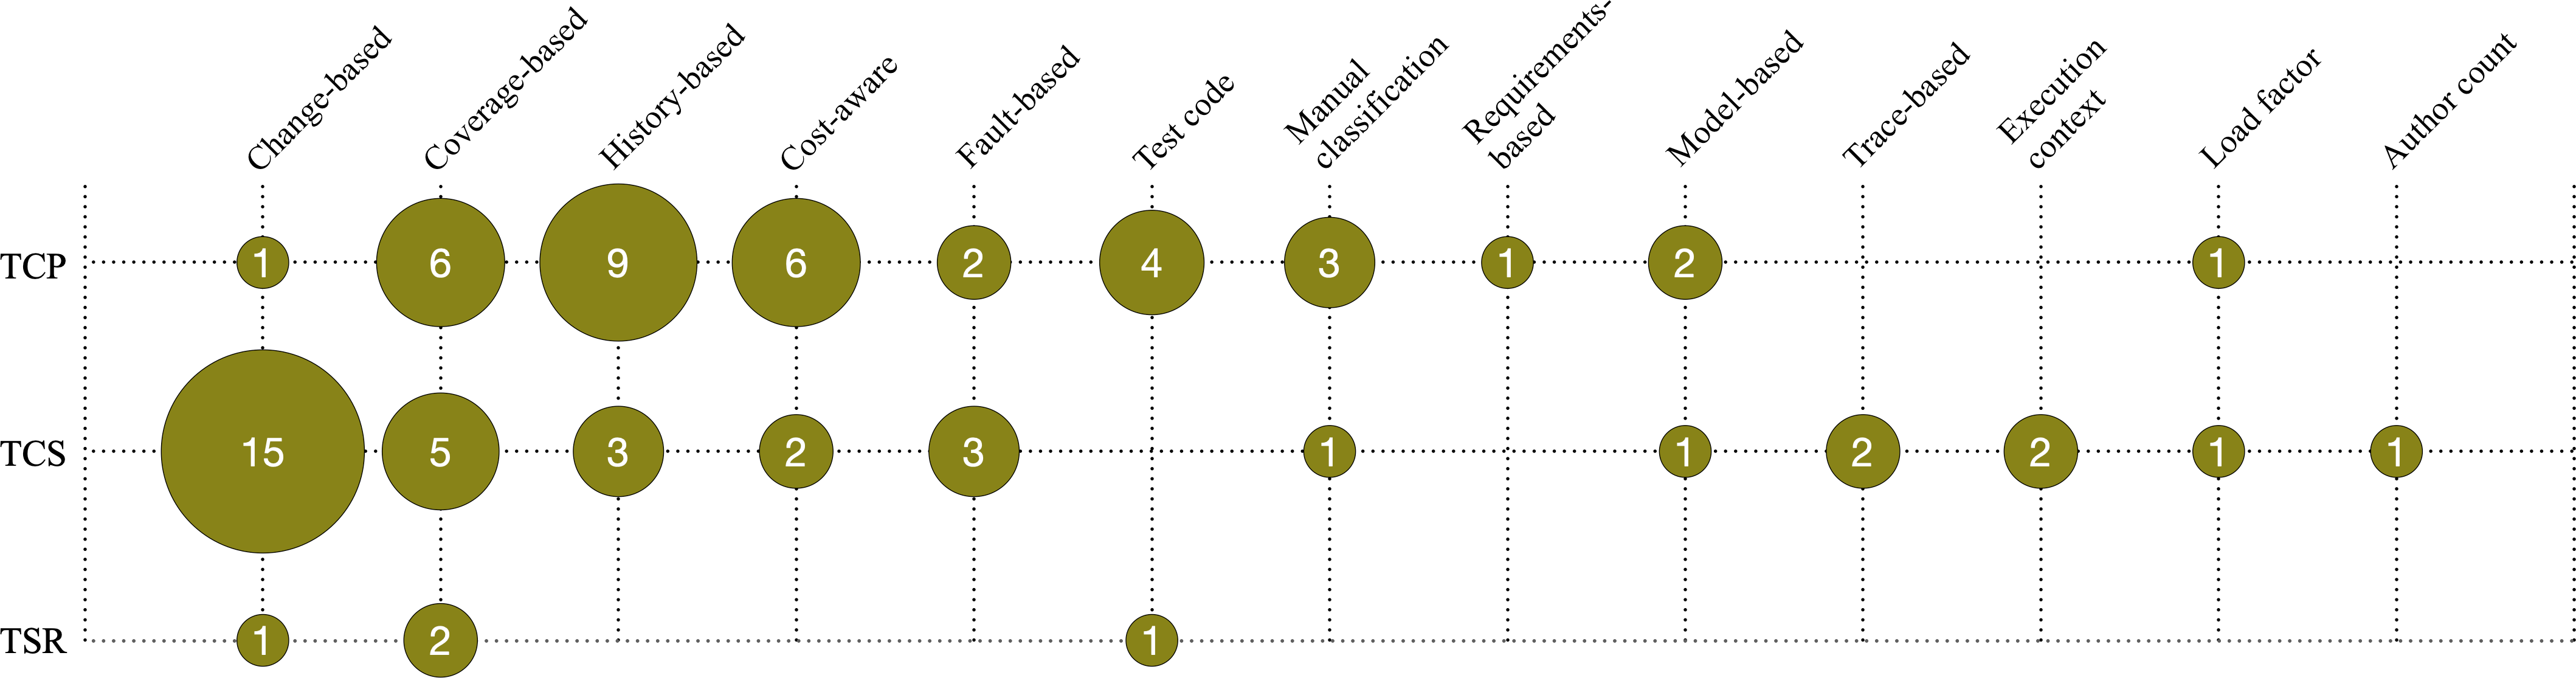
\includegraphics[width=\linewidth]{info_approach.png}
  \caption{Distribution of information approaches.}
  \label{fig:info_approaches}
\end{figure}

\begin{figure}
  \center
  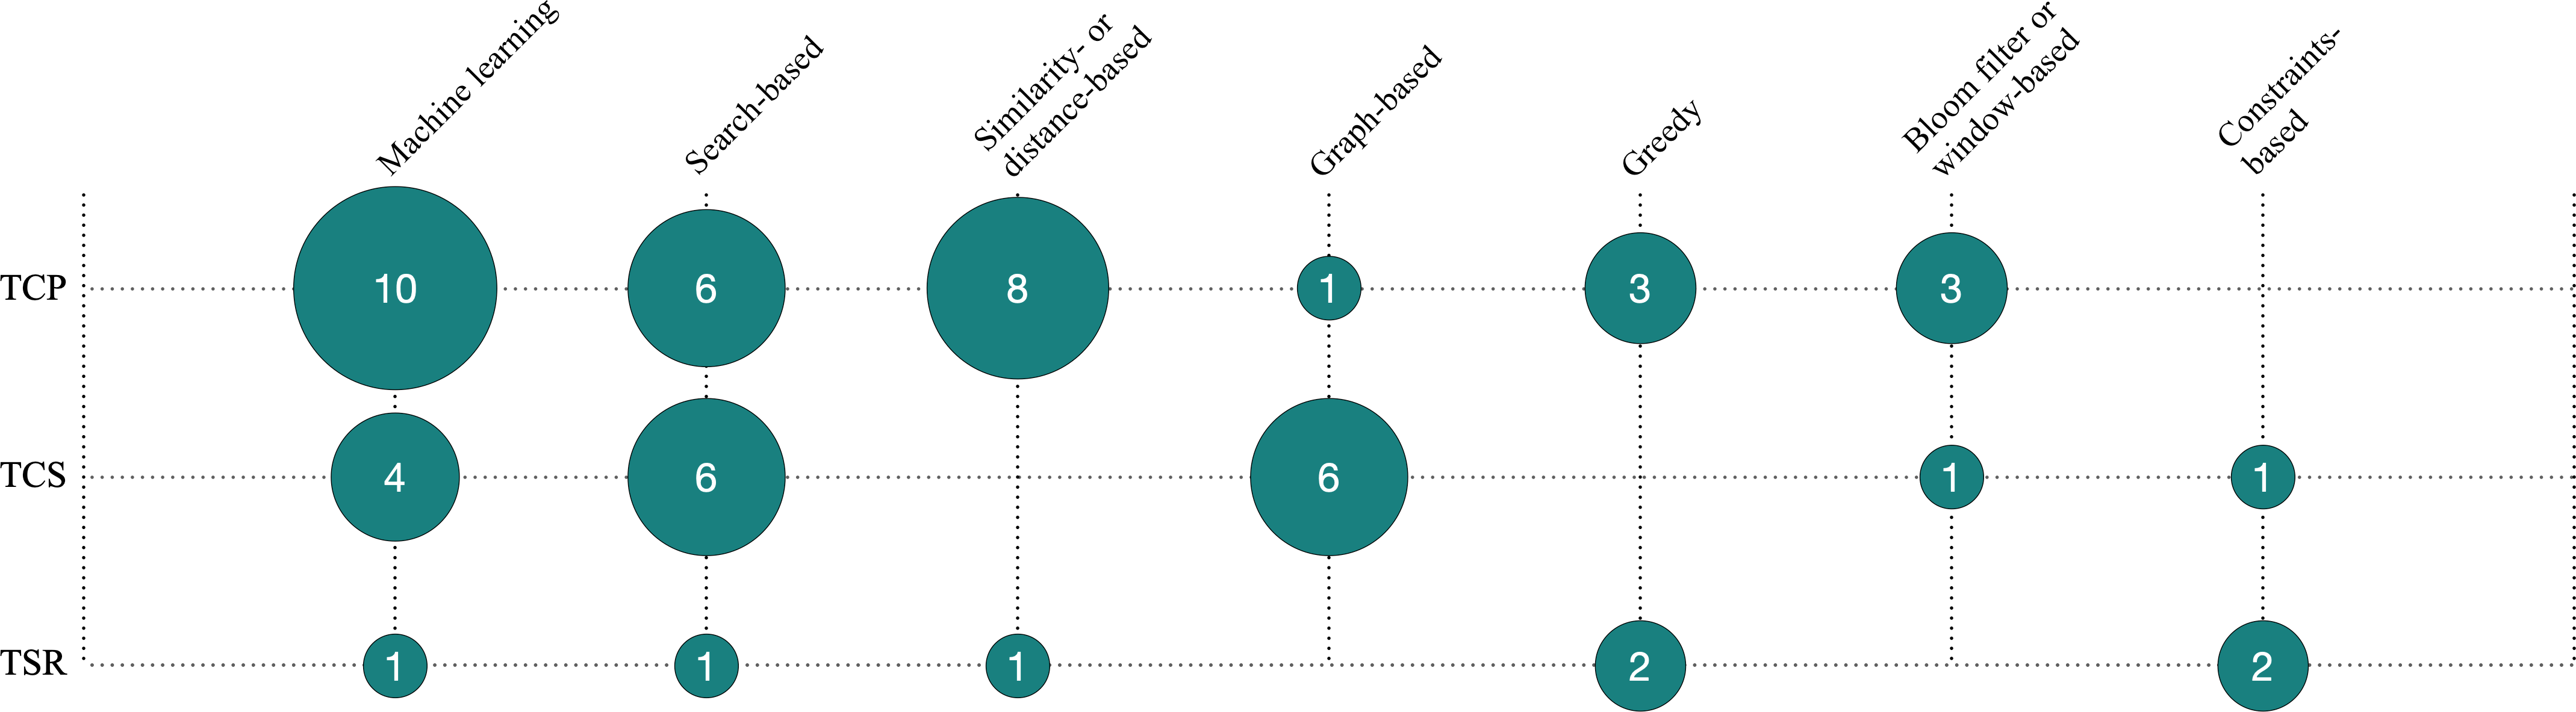
\includegraphics[width=\linewidth]{alg_approach.png}
  \caption{Distribution of algorithm approaches.}
  \label{fig:alg_approaches}
\end{figure}





\begin{table}[]
\scriptsize
\centering
\setlength{\tabcolsep}{1,2mm}
\begin{tabular}{p{23mm}p{18mm}p{18mm}p{8mm}p{3mm}p{55mm}}
\toprule
\textbf{Information} & 
\textcolor{olive}{\textbf{\tcp}} & 
\textcolor{teal}{\textbf{\tcs}} & 
\textcolor{brown}{\textbf{\tsr}} & 
\textcolor{purple}{\textbf{\tsa}} & 
\textbf{Description} \\ 
\midrule
%\rowcolors{1}{}{gray!10}
\showrowcolors
\rowapproach{History-based}{\citetalias{srikanth_test_2016}, \citetalias{aman_application_2016}, \citetalias{busjaeger_learning_2016}, \citetalias{strandberg_experience_2016}, \citetalias{marijan_effect_2016}, \citetalias{kwon_cost-effective_2017}, \citetalias{haghighatkhah_test_2018}, \citetalias{yu_terminator_2019}, \citetalias{najafi_improving_2019}}{\citetalias{kwon_cost-effective_2017}, \citetalias{machalica_predictive_2018}, \citetalias{najafi_improving_2019}}{}{}{Uses information from previous testing cycles to decide about test case relevance.}
\rowapproach{Change-based}{\citetalias{strandberg_experience_2016}}{\citetalias{oqvist_extraction-based_2016}, \citetalias{ramler_tool_2017}, \citetalias{vasic_file-level_2017}, \citetalias{celik_regression_2017}, \citetalias{zhang_hybrid_2018}, \citetalias{yilmaz_case_2018}, \citetalias{celik_regression_2018}, \citetalias{guo_decomposing_2019}, \citetalias{fu_resurgence_2019}, \citetalias{eda_efficient_2019}, \citetalias{shi_understanding_2019}, \citetalias{chen_context-aware_2021}, \citetalias{zhang_comparing_2022}, \citetalias{cingil_black-box_2022}, \citetalias{greca_comparing_2022}}{\citetalias{eda_efficient_2019}}{}{Uses changes between versions to identify the relevant test cases.}
\rowapproach{Coverage-based}{\citetalias{busjaeger_learning_2016}, \citetalias{bach_coverage-based_2017}, \citetalias{ouriques_test_2018}, \citetalias{yu_terminator_2019}, \citetalias{magalhaes_hsp_2020}, \citetalias{lubke_selecting_2020}}{\citetalias{ramler_tool_2017}, \citetalias{bach_coverage-based_2017}, \citetalias{zhong_testsage:_2019}, \citetalias{magalhaes_hsp_2020}, \citetalias{lubke_selecting_2020}}{\citetalias{shi_evaluating_2018}, \citetalias{noemmer_evaluation_2020}}{\citetalias{yoshida_fsx_2016}}{Uses structural coverage information, whereby coverage can be of statement, method, class, file, etc.}
\rowapproach{Cost-aware}{\citetalias{lu_how_2016}, \citetalias{wang_enhancing_2016}, \citetalias{tahvili_dynamic_2016}, \citetalias{tahvili_cost-benefit_2016}, \citetalias{yu_terminator_2019}, \citetalias{zhou_parallel_2022}}{\citetalias{tahvili_dynamic_2016}, \citetalias{chen_multi-objective_2021}}{}{}{Utilizes test case cost or time information to assess test relevance.}
\rowapproach{Requirements-based}{\citetalias{srikanth_requirements_2016}}{}{\citetalias{goyal_test_2019}}{}{Relate tests with project-sensitive information, such as requirements and risk assessments.}
\rowapproach{Manual classification}{\citetalias{tahvili_dynamic_2016}, \citetalias{tahvili_cost-benefit_2016}, \citetalias{yu_terminator_2019}}{\citetalias{tahvili_dynamic_2016}}{}{}{Requires at least some information that must be manually inputted by an expert.}
\rowapproach{Model-based}{\citetalias{buchgeher_improving_2016}, \citetalias{ouriques_test_2018}}{\citetalias{buchgeher_improving_2016}}{}{}{Informs the test technique using behavioural or architectural models.}
\rowapproach{Trace-based}{}{\citetalias{vost_trace-based_2016}, \citetalias{zhong_testsage:_2019}}{}{}{Provides inputs and keeps track of the effects of those inputs throughout the program.}
\rowapproach{Fault-based}{\citetalias{marijan_effect_2016}, \citetalias{zhu_test_2018}}{\citetalias{leong_assessing_2019}, \citetalias{chen_multi-objective_2021}, \citetalias{cingil_black-box_2022}}{}{}{Utilizes information related to fault detection or failure beaviour.}
\rowapproach{Test code}{\citetalias{noor_similarity-based_2016}, \citetalias{miranda_fast_2018}, \citetalias{peng_empirically_2020}, \citetalias{greca_comparing_2022}}{}{\citetalias{cruciani_scalable_2019}}{}{Uses the plain text source code of the test cases.}
\rowapproach{Load factor}{\citetalias{buchgeher_improving_2016}}{\citetalias{buchgeher_improving_2016}}{}{}{Indicates what parts of the SUT are most used by different services and components.}
\rowapproach{Author count}{}{\citetalias{leong_assessing_2019}}{}{}{Number of authors associated with a certain part of the SUT.}
\rowapproach{Execution context}{}{\citetalias{celik_regression_2017}, \citetalias{chen_context-aware_2021}}{}{}{Considers environment data such as libraries, APIs, databases, operating system, etc.}
\hiderowcolors
\bottomrule

%\end{tabular}
%\caption{Information Approaches}	
%\label{table:info_approaches}
%\end{table}
%
%
%\begin{table}[]
%\scriptsize
%\centering
%\begin{tabular}{p{25mm}p{15mm}p{15mm}p{8mm}p{8mm}p{60mm}}
%\midrule
\textbf{Algorithm} & 
\textcolor{olive}{\textbf{\tcp}} & 
\textcolor{teal}{\textbf{\tcs}} & 
\textcolor{brown}{\textbf{\tsr}} & 
\textcolor{purple}{\textbf{\tsa}} & 
\textbf{Description} \\ 
\midrule
%\rowcolors{1}{}{gray!10}
\showrowcolors
\rowapproach{Similarity or distance-based}{\citetalias{noor_similarity-based_2016}, \citetalias{aman_application_2016}, \citetalias{busjaeger_learning_2016}, \citetalias{ouriques_test_2018}, \citetalias{haghighatkhah_test_2018}, \citetalias{miranda_fast_2018}, \citetalias{zhou_beating_2020}, \citetalias{greca_comparing_2022}}{}{\citetalias{cruciani_scalable_2019}}{}{Assesses test cases based on their similarity, with the objective of diversifying the suite.}
\rowapproach{Search-based}{\citetalias{lu_how_2016}, \citetalias{wang_enhancing_2016}, \citetalias{correia_motsd_2019}, \citetalias{magalhaes_hsp_2020}, \citetalias{peng_empirically_2020}, \citetalias{zhou_parallel_2022}}{\citetalias{pradhan_search-based_2016}, \citetalias{magalhaes_automatic_2016}, \citetalias{garousi_multi-objective_2018}, \citetalias{correia_motsd_2019}, \citetalias{magalhaes_hsp_2020}, \citetalias{zarges_artificial_2021}}{\citetalias{chi_multi-level_2017}}{}{Utilizes search-based algorithms, such as genetic or nature-inspired ones}
\rowapproach{Machine learning-based}{\citetalias{busjaeger_learning_2016}, \citetalias{spieker_reinforcement_2017}, \citetalias{wu_time_2019}, \citetalias{lima_multi-armed_2022}, \citetalias{bertolino_learning--rank_2020}, \citetalias{bagherzadeh_reinforcement_2022}, \citetalias{elsner_empirically_2021}, \citetalias{abdelkarim_tcp-net_2022}, \citetalias{yaraghi_scalable_2022}, \citetalias{omri_learning_2022}}{\citetalias{machalica_predictive_2018}, \citetalias{elsner_empirically_2021}, \citetalias{mehta_data-driven_2021}, \citetalias{zhang_comparing_2022}}{\citetalias{philip_fastlane:_2019}}{}{Trains a ML model using historical or other data. Includes supervised, unsupervised and reinforcement learning methods.}
\rowapproach{Graph-based}{\citetalias{ouriques_test_2018}}{\citetalias{hirzel_graph-walk-based_2016}, \citetalias{ramler_tool_2017}, \citetalias{yilmaz_case_2018}, \citetalias{celik_regression_2018}, \citetalias{azizi_retest_2018}, \citetalias{bertolino_learning--rank_2020}}{}{}{Creates a graph representation of the SUT and utilizes graph theory algorithms to solve problems.}
\rowapproach{Greedy}{\citetalias{lu_how_2016}, \citetalias{zhou_parallel_2022}, \citetalias{li_aga_2021}}{}{\citetalias{bach_coverage-based_2017}, \citetalias{noemmer_evaluation_2020}}{}{Utilizes greedy algorithms and heuristics (usually based on coverage or similarity information).}
\rowapproach{Constraints-based}{}{\citetalias{eda_efficient_2019}}{\citetalias{gotlieb_using_2017}, \citetalias{eda_efficient_2019}}{}{Utilizes constraint programming paradigm.}
\rowapproach{Bloom filter, window-based}{\citetalias{schwartz_cost-effective_2016}, \citetalias{kwon_cost-effective_2017}, \citetalias{pan_dynamic_2020}}{\citetalias{kwon_cost-effective_2017}}{}{}{Utilizes Bloom filter data structures and time windows to filter out tests that  fail only once.}
\hiderowcolors
\bottomrule

\end{tabular}
\caption{Information- and Algorithm-based Approaches}	
\label{table:algo_approaches}
\end{table}

%\begin{table}[]
%\scriptsize
%\centering
%\rowcolors{1}{}{gray!10}
%\setlength{\tabcolsep}{5pt}
%\begin{tabular}{c|p{15mm}|p{18mm}|p{18mm}|p{5.2mm}|p{5.3mm}|p{5.3mm}|p{50mm}}
%\toprule
% & \hspace{1mm} \textbf{Metric} & \textbf{\tcp} & \textbf{\tcs} & \textbf{\tsr} & \textbf{\tsa} & \textbf{Description} \\ 
%\midrule
%\rotatebox[origin=c]{90}{\textbf{Information}} &
%\multicolumn{6}{c}{
%%	\rowcolors{1}{}{gray!10}
%	\begin{tabular}{p{15mm}|p{18mm}|p{18mm}|p{5mm}|p{5mm}|p{50mm}}
%		\showrowcolors
%		\rowapproach{History-based}{\citetalias{srikanth_test_2016}, \citetalias{aman_application_2016}, \citetalias{busjaeger_learning_2016}, \citetalias{strandberg_experience_2016}, \citetalias{marijan_effect_2016}, \citetalias{kwon_cost-effective_2017}, \citetalias{haghighatkhah_test_2018}, \citetalias{yu_terminator_2019}, \citetalias{najafi_improving_2019}}{\citetalias{kwon_cost-effective_2017}, \citetalias{machalica_predictive_2018}, \citetalias{najafi_improving_2019}}{}{}{Uses information from previous testing cycles to decide about test case relevance.}
\rowapproach{Change-based}{\citetalias{strandberg_experience_2016}}{\citetalias{oqvist_extraction-based_2016}, \citetalias{ramler_tool_2017}, \citetalias{vasic_file-level_2017}, \citetalias{celik_regression_2017}, \citetalias{zhang_hybrid_2018}, \citetalias{yilmaz_case_2018}, \citetalias{celik_regression_2018}, \citetalias{guo_decomposing_2019}, \citetalias{fu_resurgence_2019}, \citetalias{eda_efficient_2019}, \citetalias{shi_understanding_2019}, \citetalias{chen_context-aware_2021}, \citetalias{zhang_comparing_2022}, \citetalias{cingil_black-box_2022}, \citetalias{greca_comparing_2022}}{\citetalias{eda_efficient_2019}}{}{Uses changes between versions to identify the relevant test cases.}
\rowapproach{Coverage-based}{\citetalias{busjaeger_learning_2016}, \citetalias{bach_coverage-based_2017}, \citetalias{ouriques_test_2018}, \citetalias{yu_terminator_2019}, \citetalias{magalhaes_hsp_2020}, \citetalias{lubke_selecting_2020}}{\citetalias{ramler_tool_2017}, \citetalias{bach_coverage-based_2017}, \citetalias{zhong_testsage:_2019}, \citetalias{magalhaes_hsp_2020}, \citetalias{lubke_selecting_2020}}{\citetalias{shi_evaluating_2018}, \citetalias{noemmer_evaluation_2020}}{\citetalias{yoshida_fsx_2016}}{Uses structural coverage information, whereby coverage can be of statement, method, class, file, etc.}
\rowapproach{Cost-aware}{\citetalias{lu_how_2016}, \citetalias{wang_enhancing_2016}, \citetalias{tahvili_dynamic_2016}, \citetalias{tahvili_cost-benefit_2016}, \citetalias{yu_terminator_2019}, \citetalias{zhou_parallel_2022}}{\citetalias{tahvili_dynamic_2016}, \citetalias{chen_multi-objective_2021}}{}{}{Utilizes test case cost or time information to assess test relevance.}
\rowapproach{Requirements-based}{\citetalias{srikanth_requirements_2016}}{}{\citetalias{goyal_test_2019}}{}{Relate tests with project-sensitive information, such as requirements and risk assessments.}
\rowapproach{Manual classification}{\citetalias{tahvili_dynamic_2016}, \citetalias{tahvili_cost-benefit_2016}, \citetalias{yu_terminator_2019}}{\citetalias{tahvili_dynamic_2016}}{}{}{Requires at least some information that must be manually inputted by an expert.}
\rowapproach{Model-based}{\citetalias{buchgeher_improving_2016}, \citetalias{ouriques_test_2018}}{\citetalias{buchgeher_improving_2016}}{}{}{Informs the test technique using behavioural or architectural models.}
\rowapproach{Trace-based}{}{\citetalias{vost_trace-based_2016}, \citetalias{zhong_testsage:_2019}}{}{}{Provides inputs and keeps track of the effects of those inputs throughout the program.}
\rowapproach{Fault-based}{\citetalias{marijan_effect_2016}, \citetalias{zhu_test_2018}}{\citetalias{leong_assessing_2019}, \citetalias{chen_multi-objective_2021}, \citetalias{cingil_black-box_2022}}{}{}{Utilizes information related to fault detection or failure beaviour.}
\rowapproach{Test code}{\citetalias{noor_similarity-based_2016}, \citetalias{miranda_fast_2018}, \citetalias{peng_empirically_2020}, \citetalias{greca_comparing_2022}}{}{\citetalias{cruciani_scalable_2019}}{}{Uses the plain text source code of the test cases.}
\rowapproach{Load factor}{\citetalias{buchgeher_improving_2016}}{\citetalias{buchgeher_improving_2016}}{}{}{Indicates what parts of the SUT are most used by different services and components.}
\rowapproach{Author count}{}{\citetalias{leong_assessing_2019}}{}{}{Number of authors associated with a certain part of the SUT.}
\rowapproach{Execution context}{}{\citetalias{celik_regression_2017}, \citetalias{chen_context-aware_2021}}{}{}{Considers environment data such as libraries, APIs, databases, operating system, etc.}
\hiderowcolors
\bottomrule

%		
%
%	\end{tabular}
%}\\
%\midrule
%\rotatebox[origin=c]{90}{\textbf{Algorithm}} &
%\multicolumn{6}{c}{
%%	\rowcolors{1}{}{gray!10}
%	\begin{tabular}{p{15mm}p{18mm}p{18mm}p{5mm}p{5mm}p{50mm}}
%		\showrowcolors
%		\rowapproach{Similarity or distance-based}{\citetalias{noor_similarity-based_2016}, \citetalias{aman_application_2016}, \citetalias{busjaeger_learning_2016}, \citetalias{ouriques_test_2018}, \citetalias{haghighatkhah_test_2018}, \citetalias{miranda_fast_2018}, \citetalias{zhou_beating_2020}, \citetalias{greca_comparing_2022}}{}{\citetalias{cruciani_scalable_2019}}{}{Assesses test cases based on their similarity, with the objective of diversifying the suite.}
\rowapproach{Search-based}{\citetalias{lu_how_2016}, \citetalias{wang_enhancing_2016}, \citetalias{correia_motsd_2019}, \citetalias{magalhaes_hsp_2020}, \citetalias{peng_empirically_2020}, \citetalias{zhou_parallel_2022}}{\citetalias{pradhan_search-based_2016}, \citetalias{magalhaes_automatic_2016}, \citetalias{garousi_multi-objective_2018}, \citetalias{correia_motsd_2019}, \citetalias{magalhaes_hsp_2020}, \citetalias{zarges_artificial_2021}}{\citetalias{chi_multi-level_2017}}{}{Utilizes search-based algorithms, such as genetic or nature-inspired ones}
\rowapproach{Machine learning-based}{\citetalias{busjaeger_learning_2016}, \citetalias{spieker_reinforcement_2017}, \citetalias{wu_time_2019}, \citetalias{lima_multi-armed_2022}, \citetalias{bertolino_learning--rank_2020}, \citetalias{bagherzadeh_reinforcement_2022}, \citetalias{elsner_empirically_2021}, \citetalias{abdelkarim_tcp-net_2022}, \citetalias{yaraghi_scalable_2022}, \citetalias{omri_learning_2022}}{\citetalias{machalica_predictive_2018}, \citetalias{elsner_empirically_2021}, \citetalias{mehta_data-driven_2021}, \citetalias{zhang_comparing_2022}}{\citetalias{philip_fastlane:_2019}}{}{Trains a ML model using historical or other data. Includes supervised, unsupervised and reinforcement learning methods.}
\rowapproach{Graph-based}{\citetalias{ouriques_test_2018}}{\citetalias{hirzel_graph-walk-based_2016}, \citetalias{ramler_tool_2017}, \citetalias{yilmaz_case_2018}, \citetalias{celik_regression_2018}, \citetalias{azizi_retest_2018}, \citetalias{bertolino_learning--rank_2020}}{}{}{Creates a graph representation of the SUT and utilizes graph theory algorithms to solve problems.}
\rowapproach{Greedy}{\citetalias{lu_how_2016}, \citetalias{zhou_parallel_2022}, \citetalias{li_aga_2021}}{}{\citetalias{bach_coverage-based_2017}, \citetalias{noemmer_evaluation_2020}}{}{Utilizes greedy algorithms and heuristics (usually based on coverage or similarity information).}
\rowapproach{Constraints-based}{}{\citetalias{eda_efficient_2019}}{\citetalias{gotlieb_using_2017}, \citetalias{eda_efficient_2019}}{}{Utilizes constraint programming paradigm.}
\rowapproach{Bloom filter, window-based}{\citetalias{schwartz_cost-effective_2016}, \citetalias{kwon_cost-effective_2017}, \citetalias{pan_dynamic_2020}}{\citetalias{kwon_cost-effective_2017}}{}{}{Utilizes Bloom filter data structures and time windows to filter out tests that  fail only once.}
\hiderowcolors
\bottomrule

%		
%	\end{tabular}
%}\\
%
%\bottomrule
%
%\end{tabular}
%\caption{Approaches}	
%\label{table:approaches}
%\end{table}

The main metrics reported in the literature are shown in \autoref{table:other_metrics}, \autoref{fig:effectiveness_metrics} and \autoref{fig:efficiency_metrics}, grouped according to their main goal\footnote{In each figure, we omit \tsa due to space concerns, as only one paper~\citepalias{yoshida_fsx_2016} covers it.}.
The reported metrics primarily focus on effectiveness (how good a solution is at accomplishing its task) or efficiency (the time and cost of using the solution), but two metrics were identified that are neither --- namely, applicability/generality and diagnosability.

APFD is the most widely accepted metric for assessing \tcp{} approaches.
Because \tcs and \tsr both have the goal of running fewer tests than an original test suite, their metrics are mostly shared: testing time, selection count and fault detection ability are the most common ones.
The set of accuracy/precision/recall appears to be the effectiveness metric that covers the most situations.
For efficiency, the execution time of a technique is both widely used and is useful for any kind of solution.

%\newcommand{\rowmetric}[6]{
#1 & % Name
\textcolor{verdun}{#2} & % TCP
\textcolor{cyprus}{#3} & % TCS
\textcolor{derby}{#4} & % TSR
\textcolor{bossanova}{#5} & % TSA
#6 % Description
\\}

\begin{figure}
  \center
  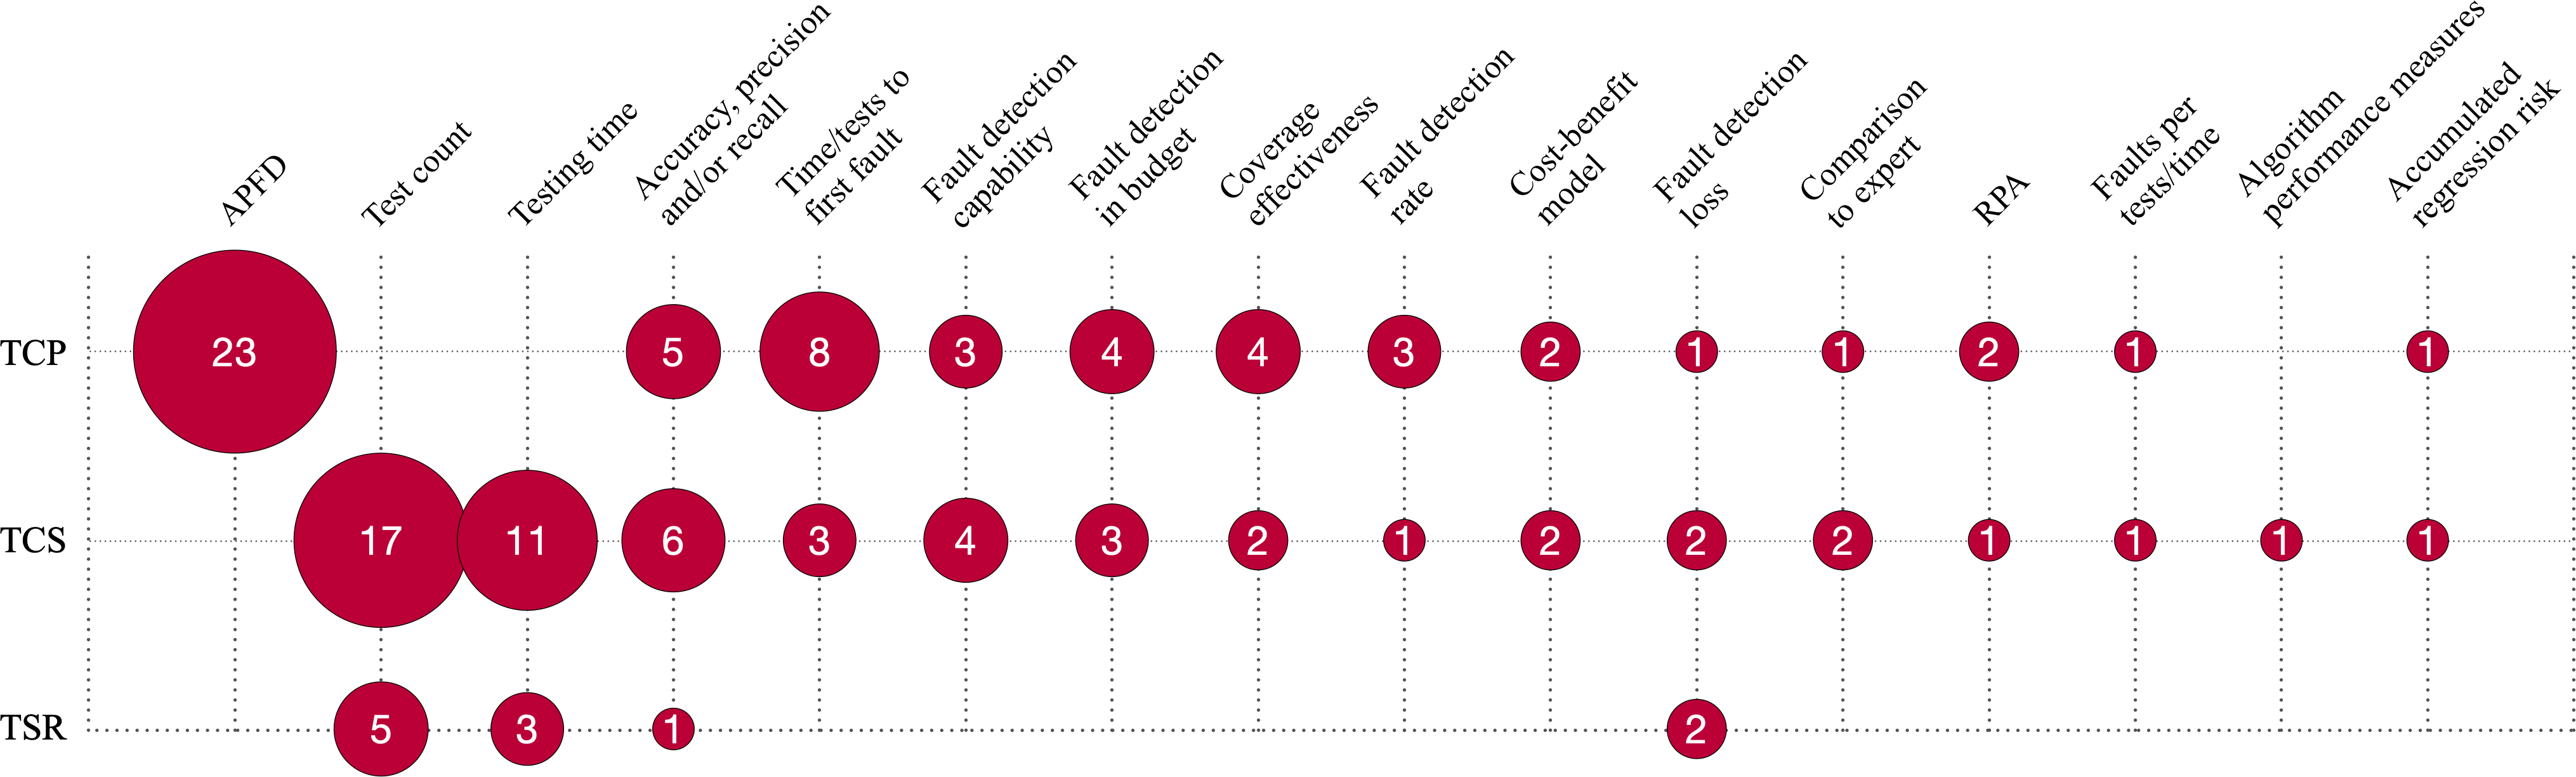
\includegraphics[width=\linewidth]{figures/effectiveness_metrics.pdf}
  \caption{Distribution of effectiveness metrics.}
  \label{fig:effectiveness_metrics}
\end{figure}

\begin{figure}
  \center
  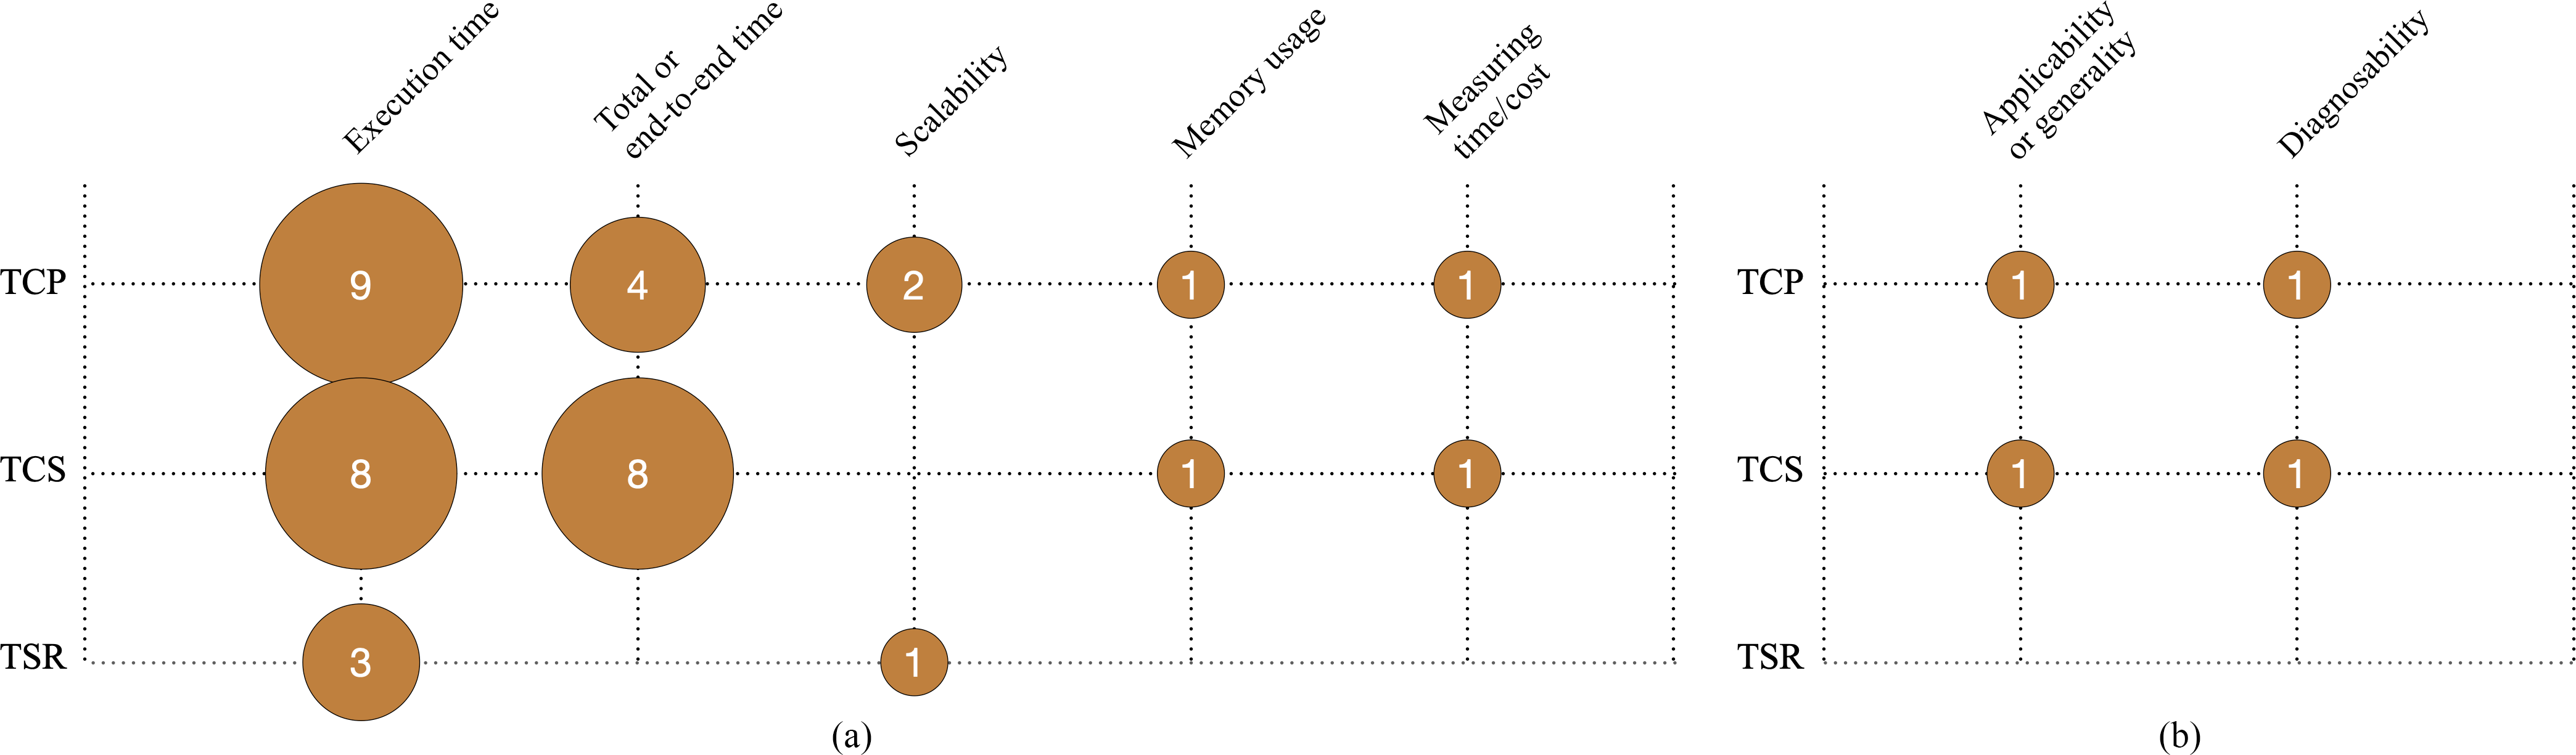
\includegraphics[width=\linewidth]{figures/efficiency_other_metrics.pdf}
  \caption{Distribution of (a) efficiency and (b) other metrics.}
  \label{fig:efficiency_metrics}
\end{figure}

\begin{table}[]
\scriptsize
\centering
\setlength{\tabcolsep}{1,2mm}
\begin{tabular}{p{23mm}p{18mm}p{18mm}p{8mm}p{8mm}p{60mm}}
\toprule
\textbf{Effectiveness} & 
\textcolor{verdun}{\textbf{\tcp}} & 
\textcolor{cyprus}{\textbf{\tcs}} & 
\textcolor{derby}{\textbf{\tsr}} & 
\textcolor{bossanova}{\textbf{\tsa}} & 
\textbf{Description} \\ 
\midrule
\showrowcolors
\rowmetric{Selection/reduction count/percentage}{}{\citetalias{hirzel_graph-walk-based_2016}, \citetalias{vost_trace-based_2016}, \citetalias{blondeau_test_2017}, \citetalias{bach_coverage-based_2017}, \citetalias{vasic_file-level_2017}, \citetalias{celik_regression_2017}, \citetalias{zhang_hybrid_2018}, \citetalias{yilmaz_case_2018}, \citetalias{celik_regression_2018}, \citetalias{azizi_retest_2018}, \citetalias{fu_resurgence_2019}, \citetalias{eda_efficient_2019}, \citetalias{machalica_predictive_2018}, \citetalias{shi_understanding_2019}, \citetalias{chen_context-aware_2021}, \citetalias{zhang_comparing_2022}, \citetalias{cingil_black-box_2022}}{\citetalias{gotlieb_using_2017}, \citetalias{chi_multi-level_2017}, \citetalias{eda_efficient_2019}, \citetalias{goyal_test_2019}, \citetalias{noemmer_evaluation_2020}}{}{Absolute or relative size of the resulting test suite compared to the original.}
\rowmetric{Average Percentage of Faults Detected (APFD)}{\citetalias{srikanth_requirements_2016}, \citetalias{lu_how_2016}, \citetalias{srikanth_test_2016}, \citetalias{busjaeger_learning_2016}, \citetalias{marijan_effect_2016}, \citetalias{spieker_reinforcement_2017}, \citetalias{ouriques_test_2018}, \citetalias{haghighatkhah_test_2018}, \citetalias{miranda_fast_2018}, \citetalias{chen_optimizing_2018}, \citetalias{yu_terminator_2019}, \citetalias{wu_time_2019}, \citetalias{lima_multi-armed_2022}, \citetalias{peng_empirically_2020}, \citetalias{bagherzadeh_reinforcement_2022}, \citetalias{pan_dynamic_2020}, \citetalias{zhou_parallel_2022}, \citetalias{li_aga_2021}, \citetalias{abdelkarim_tcp-net_2022}, \citetalias{yaraghi_scalable_2022}, \citetalias{omri_learning_2022}, \citetalias{greca_comparing_2022}}{}{}{}{A measure of how quickly a test suite detects faults, on average. Includes many variations, such as APFDc and NAPFD.}
\rowmetric{Testing time}{}{\citetalias{tahvili_dynamic_2016}, \citetalias{ramler_tool_2017}, \citetalias{celik_regression_2017}, \citetalias{garousi_multi-objective_2018}, \citetalias{yilmaz_case_2018}, \citetalias{celik_regression_2018}, \citetalias{zhong_testsage:_2019}, \citetalias{shi_understanding_2019}, \citetalias{mehta_data-driven_2021}, \citetalias{zhang_comparing_2022}, \citetalias{cingil_black-box_2022}}{\citetalias{goyal_test_2019}, \citetalias{philip_fastlane:_2019}, \citetalias{noemmer_evaluation_2020}}{}{Time required to execute the prioritized/selected/reduced test suite as opposed to the original suite.}
\rowmetric{Accuracy, precision and recall}{\citetalias{busjaeger_learning_2016}, \citetalias{kwon_cost-effective_2017}, \citetalias{pan_dynamic_2020}, \citetalias{abdelkarim_tcp-net_2022}, \citetalias{omri_learning_2022}}{\citetalias{blondeau_test_2017}, \citetalias{magalhaes_automatic_2016}, \citetalias{kwon_cost-effective_2017}, \citetalias{guo_decomposing_2019}, \citetalias{machalica_predictive_2018}, \citetalias{xu_requirement-based_2021}}{\citetalias{philip_fastlane:_2019}}{}{Measures of correctness and completeness of the resulting test suite (e.g., count of false positives and false negatives).}
\rowmetric{Fault Detection Capability}{\citetalias{schwartz_cost-effective_2016}, \citetalias{wang_enhancing_2016}, \citetalias{marijan_effect_2016}}{\citetalias{kwon_cost-effective_2017}, \citetalias{zarges_artificial_2021}, \citetalias{chen_context-aware_2021}, \citetalias{cingil_black-box_2022}}{}{}{Number or proportion of faults detected by the resulting suite compared to the original.}
\rowmetric{Fault Detection Rate (FDR)}{\citetalias{aman_application_2016}, \citetalias{strandberg_experience_2016}, \citetalias{yu_terminator_2019}}{\citetalias{azizi_retest_2018}}{}{}{Time to detect faults compared to the optimal RT suite.}
\rowmetric{Coverage Effectiveness (CE)}{\citetalias{noor_similarity-based_2016}, \citetalias{yu_terminator_2019}, \citetalias{magalhaes_hsp_2020}, \citetalias{lubke_selecting_2020}}{\citetalias{magalhaes_hsp_2020}, \citetalias{lubke_selecting_2020}}{}{\citetalias{yoshida_fsx_2016}}{Measure of the tradeoff between cost of the test suite and structural coverage of the SUT.}
\rowmetric{Time/tests To First Failure}{\citetalias{noor_similarity-based_2016}, \citetalias{chen_optimizing_2018}, \citetalias{zhu_test_2018}, \citetalias{lima_multi-armed_2022}, \citetalias{zhou_beating_2020}, \citetalias{pan_dynamic_2020}, \citetalias{zhou_parallel_2022}, \citetalias{greca_comparing_2022}}{\citetalias{blondeau_test_2017}, \citetalias{zarges_artificial_2021}, \citetalias{greca_comparing_2022}}{}{}{Number of tests or amount of time needed to reach the first failure.}
\rowmetric{Fault detection within a budget}{\citetalias{wang_enhancing_2016}, \citetalias{bach_coverage-based_2017}, \citetalias{lima_multi-armed_2022}, \citetalias{greca_comparing_2022}}{\citetalias{pradhan_search-based_2016}, \citetalias{bach_coverage-based_2017}, \citetalias{greca_comparing_2022}}{}{}{Faults still detected when restricting the testing time budget.}
\rowmetric{Cost-benefit model}{\citetalias{schwartz_cost-effective_2016}, \citetalias{tahvili_cost-benefit_2016}}{\citetalias{garousi_multi-objective_2018}, \citetalias{mehta_data-driven_2021}}{}{}{Mathematical models considering costs and benefits of applying a technique throughout development.}
\rowmetric{Fault Detection Loss}{\citetalias{najafi_improving_2019}}{\citetalias{najafi_improving_2019}, \citetalias{chen_multi-objective_2021}}{\citetalias{shi_evaluating_2018}, \citetalias{cruciani_scalable_2019}}{}{Number or proportion of faults undetected by the selected/reduced test suite compared to the original.}
\rowmetric{Comparison to expert}{\citetalias{buchgeher_improving_2016}}{\citetalias{buchgeher_improving_2016}, \citetalias{magalhaes_automatic_2016}}{}{}{Compares the output of the tool with a list of tests selected by the project architect.}
\rowmetric{Faults per tests or time}{\citetalias{kwon_cost-effective_2017}}{\citetalias{kwon_cost-effective_2017}}{}{}{Number of faults deteted per number of tests or testing time.}
\rowmetric{Number of tests added}{}{}{}{\citetalias{yoshida_fsx_2016}}{Number of tests added to the test suite.}
\rowmetric{Algorithm performance measures}{}{\citetalias{pradhan_search-based_2016}}{}{}{Fitness value or hypervolume metrics applied to search-based algorithms}
\rowmetric{Accumulated regression risk}{\citetalias{lubke_selecting_2020}}{\citetalias{lubke_selecting_2020}}{}{}{How much of the "regression risk" is covered by the tests.}
\rowmetric{Rank Percentile Average (RPA)}{\citetalias{bertolino_learning--rank_2020}, \citetalias{bagherzadeh_reinforcement_2022}}{\citetalias{bertolino_learning--rank_2020}}{}{}{Comparison between the predicted ranking and the actual ranking (from the dataset).}
\hiderowcolors
\bottomrule

%\end{tabular}
%\caption{Effectiveness Metrics}	
%\label{table:effectiveness_metrics}
%\end{table}
%
%\begin{table}[]
%\scriptsize
%\centering
%\begin{tabular}{p{25mm}p{15mm}p{15mm}p{8mm}p{8mm}p{60mm}}
%\toprule
\textbf{Efficiency} & 
\textcolor{verdun}{\textbf{\tcp}} & 
\textcolor{cyprus}{\textbf{\tcs}} & 
\textcolor{derby}{\textbf{\tsr}} & 
\textcolor{bossanova}{\textbf{\tsa}} & 
\textbf{Description} \\ \midrule
\showrowcolors
\rowmetric{Execution time}{\citetalias{wang_enhancing_2016}, \citetalias{haghighatkhah_test_2018}, \citetalias{miranda_fast_2018}, \citetalias{najafi_improving_2019}, \citetalias{wu_time_2019}, \citetalias{lima_multi-armed_2022}, \citetalias{zhou_parallel_2022}, \citetalias{li_aga_2021}, \citetalias{greca_comparing_2022}}{\citetalias{hirzel_graph-walk-based_2016}, \citetalias{vasic_file-level_2017}, \citetalias{celik_regression_2017}, \citetalias{zhong_testsage:_2019}, \citetalias{najafi_improving_2019}, \citetalias{xu_requirement-based_2021}, \citetalias{zhang_comparing_2022}, \citetalias{greca_comparing_2022}}{\citetalias{gotlieb_using_2017}, \citetalias{chi_multi-level_2017}, \citetalias{cruciani_scalable_2019}}{\citetalias{yoshida_fsx_2016}}{Time required to run the tool (e.g., selection time, prioritization time, etc).}
\rowmetric{Total/End-to-end time}{\citetalias{wang_enhancing_2016}, \citetalias{miranda_fast_2018}, \citetalias{bertolino_learning--rank_2020}, \citetalias{greca_comparing_2022}}{\citetalias{oqvist_extraction-based_2016}, \citetalias{vasic_file-level_2017}, \citetalias{zhang_hybrid_2018}, \citetalias{celik_regression_2018}, \citetalias{fu_resurgence_2019}, \citetalias{bertolino_learning--rank_2020}, \citetalias{zhang_comparing_2022}, \citetalias{greca_comparing_2022}}{}{}{End-to-end time, combining measuring time, execution time and testing time. Due to this, it is a measure of both efficiency and effectiveness.}
\rowmetric{Memory usage}{\citetalias{wang_enhancing_2016}}{\citetalias{hirzel_graph-walk-based_2016}}{}{}{Measures the amount of memory used by the tool.}
\rowmetric{Scalability}{\citetalias{miranda_fast_2018}, \citetalias{yaraghi_scalable_2022}}{}{\citetalias{cruciani_scalable_2019}}{}{How well the tool performs on subjects of different sizes.}
\rowmetric{Measuring time/cost}{\citetalias{elsner_empirically_2021}}{\citetalias{elsner_empirically_2021}}{}{}{Measure of how costly is the information needed by the technique (e.g. compiling tests, collecting coverage, training a model).}
\hiderowcolors
\bottomrule

%\end{tabular}
%\caption{Efficiency Metrics}	
%\label{table:efficiency_metrics}
%\end{table}
%
%\begin{table}[]
%\scriptsize
%\centering
%\begin{tabular}{p{25mm}p{15mm}p{15mm}p{8mm}p{8mm}p{60mm}}
%\toprule
\textbf{Other} & 
\textcolor{verdun}{\textbf{\tcp}} & 
\textcolor{cyprus}{\textbf{\tcs}} & 
\textcolor{derby}{\textbf{\tsr}} & 
\textcolor{bossanova}{\textbf{\tsa}} & 
\textbf{Description} \\ \midrule
\showrowcolors
\rowmetric{Applicability/Generality}{\citetalias{zhou_beating_2020}}{\citetalias{xu_requirement-based_2021}}{}{}{The variety of SUTs upon which the tool can be applied.}
\rowmetric{Diagnosability}{\citetalias{correia_motsd_2019}}{\citetalias{correia_motsd_2019}}{}{}{Cost of diagnosing a fault upon detection.}
\hiderowcolors
\bottomrule

\end{tabular}
\caption{Effectiveness, Efficiency and Other Metrics}	
\label{table:other_metrics}
\end{table}

\setlength{\tabcolsep}{6pt}

%\begin{table}[h]
%\scriptsize
%\centering
%\begin{tabular}{cp{42mm}p{22mm}p{5.2mm}p{5.2mm}p{5.2mm}p{5.3mm}p{50mm}}
%\toprule
% & \hspace{1mm} \textbf{Metric} & \textbf{Referenced in} & \textbf{\tcp} & \textbf{\tcs} & \textbf{\tsr} & \textbf{\tsa} & \textbf{Description} \\ 
%\midrule
%
%\rotatebox[origin=c]{90}{\textbf{Effectiveness}} &
%\multicolumn{6}{c}{
%	\rowcolors{1}{}{gray!10}
%	\begin{tabular}{p{40mm}p{23mm}p{5mm}p{5mm}p{5mm}p{5mm}p{50mm}}
%	
%	\rowmetric{Selection/reduction count/percentage}{}{\citetalias{hirzel_graph-walk-based_2016}, \citetalias{vost_trace-based_2016}, \citetalias{blondeau_test_2017}, \citetalias{bach_coverage-based_2017}, \citetalias{vasic_file-level_2017}, \citetalias{celik_regression_2017}, \citetalias{zhang_hybrid_2018}, \citetalias{yilmaz_case_2018}, \citetalias{celik_regression_2018}, \citetalias{azizi_retest_2018}, \citetalias{fu_resurgence_2019}, \citetalias{eda_efficient_2019}, \citetalias{machalica_predictive_2018}, \citetalias{shi_understanding_2019}, \citetalias{chen_context-aware_2021}, \citetalias{zhang_comparing_2022}, \citetalias{cingil_black-box_2022}}{\citetalias{gotlieb_using_2017}, \citetalias{chi_multi-level_2017}, \citetalias{eda_efficient_2019}, \citetalias{goyal_test_2019}, \citetalias{noemmer_evaluation_2020}}{}{Absolute or relative size of the resulting test suite compared to the original.}
\rowmetric{Average Percentage of Faults Detected (APFD)}{\citetalias{srikanth_requirements_2016}, \citetalias{lu_how_2016}, \citetalias{srikanth_test_2016}, \citetalias{busjaeger_learning_2016}, \citetalias{marijan_effect_2016}, \citetalias{spieker_reinforcement_2017}, \citetalias{ouriques_test_2018}, \citetalias{haghighatkhah_test_2018}, \citetalias{miranda_fast_2018}, \citetalias{chen_optimizing_2018}, \citetalias{yu_terminator_2019}, \citetalias{wu_time_2019}, \citetalias{lima_multi-armed_2022}, \citetalias{peng_empirically_2020}, \citetalias{bagherzadeh_reinforcement_2022}, \citetalias{pan_dynamic_2020}, \citetalias{zhou_parallel_2022}, \citetalias{li_aga_2021}, \citetalias{abdelkarim_tcp-net_2022}, \citetalias{yaraghi_scalable_2022}, \citetalias{omri_learning_2022}, \citetalias{greca_comparing_2022}}{}{}{}{A measure of how quickly a test suite detects faults, on average. Includes many variations, such as APFDc and NAPFD.}
\rowmetric{Testing time}{}{\citetalias{tahvili_dynamic_2016}, \citetalias{ramler_tool_2017}, \citetalias{celik_regression_2017}, \citetalias{garousi_multi-objective_2018}, \citetalias{yilmaz_case_2018}, \citetalias{celik_regression_2018}, \citetalias{zhong_testsage:_2019}, \citetalias{shi_understanding_2019}, \citetalias{mehta_data-driven_2021}, \citetalias{zhang_comparing_2022}, \citetalias{cingil_black-box_2022}}{\citetalias{goyal_test_2019}, \citetalias{philip_fastlane:_2019}, \citetalias{noemmer_evaluation_2020}}{}{Time required to execute the prioritized/selected/reduced test suite as opposed to the original suite.}
\rowmetric{Accuracy, precision and recall}{\citetalias{busjaeger_learning_2016}, \citetalias{kwon_cost-effective_2017}, \citetalias{pan_dynamic_2020}, \citetalias{abdelkarim_tcp-net_2022}, \citetalias{omri_learning_2022}}{\citetalias{blondeau_test_2017}, \citetalias{magalhaes_automatic_2016}, \citetalias{kwon_cost-effective_2017}, \citetalias{guo_decomposing_2019}, \citetalias{machalica_predictive_2018}, \citetalias{xu_requirement-based_2021}}{\citetalias{philip_fastlane:_2019}}{}{Measures of correctness and completeness of the resulting test suite (e.g., count of false positives and false negatives).}
\rowmetric{Fault Detection Capability}{\citetalias{schwartz_cost-effective_2016}, \citetalias{wang_enhancing_2016}, \citetalias{marijan_effect_2016}}{\citetalias{kwon_cost-effective_2017}, \citetalias{zarges_artificial_2021}, \citetalias{chen_context-aware_2021}, \citetalias{cingil_black-box_2022}}{}{}{Number or proportion of faults detected by the resulting suite compared to the original.}
\rowmetric{Fault Detection Rate (FDR)}{\citetalias{aman_application_2016}, \citetalias{strandberg_experience_2016}, \citetalias{yu_terminator_2019}}{\citetalias{azizi_retest_2018}}{}{}{Time to detect faults compared to the optimal RT suite.}
\rowmetric{Coverage Effectiveness (CE)}{\citetalias{noor_similarity-based_2016}, \citetalias{yu_terminator_2019}, \citetalias{magalhaes_hsp_2020}, \citetalias{lubke_selecting_2020}}{\citetalias{magalhaes_hsp_2020}, \citetalias{lubke_selecting_2020}}{}{\citetalias{yoshida_fsx_2016}}{Measure of the tradeoff between cost of the test suite and structural coverage of the SUT.}
\rowmetric{Time/tests To First Failure}{\citetalias{noor_similarity-based_2016}, \citetalias{chen_optimizing_2018}, \citetalias{zhu_test_2018}, \citetalias{lima_multi-armed_2022}, \citetalias{zhou_beating_2020}, \citetalias{pan_dynamic_2020}, \citetalias{zhou_parallel_2022}, \citetalias{greca_comparing_2022}}{\citetalias{blondeau_test_2017}, \citetalias{zarges_artificial_2021}, \citetalias{greca_comparing_2022}}{}{}{Number of tests or amount of time needed to reach the first failure.}
\rowmetric{Fault detection within a budget}{\citetalias{wang_enhancing_2016}, \citetalias{bach_coverage-based_2017}, \citetalias{lima_multi-armed_2022}, \citetalias{greca_comparing_2022}}{\citetalias{pradhan_search-based_2016}, \citetalias{bach_coverage-based_2017}, \citetalias{greca_comparing_2022}}{}{}{Faults still detected when restricting the testing time budget.}
\rowmetric{Cost-benefit model}{\citetalias{schwartz_cost-effective_2016}, \citetalias{tahvili_cost-benefit_2016}}{\citetalias{garousi_multi-objective_2018}, \citetalias{mehta_data-driven_2021}}{}{}{Mathematical models considering costs and benefits of applying a technique throughout development.}
\rowmetric{Fault Detection Loss}{\citetalias{najafi_improving_2019}}{\citetalias{najafi_improving_2019}, \citetalias{chen_multi-objective_2021}}{\citetalias{shi_evaluating_2018}, \citetalias{cruciani_scalable_2019}}{}{Number or proportion of faults undetected by the selected/reduced test suite compared to the original.}
\rowmetric{Comparison to expert}{\citetalias{buchgeher_improving_2016}}{\citetalias{buchgeher_improving_2016}, \citetalias{magalhaes_automatic_2016}}{}{}{Compares the output of the tool with a list of tests selected by the project architect.}
\rowmetric{Faults per tests or time}{\citetalias{kwon_cost-effective_2017}}{\citetalias{kwon_cost-effective_2017}}{}{}{Number of faults deteted per number of tests or testing time.}
\rowmetric{Number of tests added}{}{}{}{\citetalias{yoshida_fsx_2016}}{Number of tests added to the test suite.}
\rowmetric{Algorithm performance measures}{}{\citetalias{pradhan_search-based_2016}}{}{}{Fitness value or hypervolume metrics applied to search-based algorithms}
\rowmetric{Accumulated regression risk}{\citetalias{lubke_selecting_2020}}{\citetalias{lubke_selecting_2020}}{}{}{How much of the "regression risk" is covered by the tests.}
\rowmetric{Rank Percentile Average (RPA)}{\citetalias{bertolino_learning--rank_2020}, \citetalias{bagherzadeh_reinforcement_2022}}{\citetalias{bertolino_learning--rank_2020}}{}{}{Comparison between the predicted ranking and the actual ranking (from the dataset).}
\hiderowcolors
\bottomrule

%	
%	\end{tabular}
%}\\
%\midrule
%\rotatebox[origin=c]{90}{\textbf{Efficiency}} &
%\multicolumn{6}{c}{
%	\rowcolors{1}{}{gray!10}
%	\begin{tabular}{p{40mm}p{23mm}p{5mm}p{5mm}p{5mm}p{5mm}p{50mm}}
%	
%	\rowmetric{Execution time}{\citetalias{wang_enhancing_2016}, \citetalias{haghighatkhah_test_2018}, \citetalias{miranda_fast_2018}, \citetalias{najafi_improving_2019}, \citetalias{wu_time_2019}, \citetalias{lima_multi-armed_2022}, \citetalias{zhou_parallel_2022}, \citetalias{li_aga_2021}, \citetalias{greca_comparing_2022}}{\citetalias{hirzel_graph-walk-based_2016}, \citetalias{vasic_file-level_2017}, \citetalias{celik_regression_2017}, \citetalias{zhong_testsage:_2019}, \citetalias{najafi_improving_2019}, \citetalias{xu_requirement-based_2021}, \citetalias{zhang_comparing_2022}, \citetalias{greca_comparing_2022}}{\citetalias{gotlieb_using_2017}, \citetalias{chi_multi-level_2017}, \citetalias{cruciani_scalable_2019}}{\citetalias{yoshida_fsx_2016}}{Time required to run the tool (e.g., selection time, prioritization time, etc).}
\rowmetric{Total/End-to-end time}{\citetalias{wang_enhancing_2016}, \citetalias{miranda_fast_2018}, \citetalias{bertolino_learning--rank_2020}, \citetalias{greca_comparing_2022}}{\citetalias{oqvist_extraction-based_2016}, \citetalias{vasic_file-level_2017}, \citetalias{zhang_hybrid_2018}, \citetalias{celik_regression_2018}, \citetalias{fu_resurgence_2019}, \citetalias{bertolino_learning--rank_2020}, \citetalias{zhang_comparing_2022}, \citetalias{greca_comparing_2022}}{}{}{End-to-end time, combining measuring time, execution time and testing time. Due to this, it is a measure of both efficiency and effectiveness.}
\rowmetric{Memory usage}{\citetalias{wang_enhancing_2016}}{\citetalias{hirzel_graph-walk-based_2016}}{}{}{Measures the amount of memory used by the tool.}
\rowmetric{Scalability}{\citetalias{miranda_fast_2018}, \citetalias{yaraghi_scalable_2022}}{}{\citetalias{cruciani_scalable_2019}}{}{How well the tool performs on subjects of different sizes.}
\rowmetric{Measuring time/cost}{\citetalias{elsner_empirically_2021}}{\citetalias{elsner_empirically_2021}}{}{}{Measure of how costly is the information needed by the technique (e.g. compiling tests, collecting coverage, training a model).}
\hiderowcolors
\bottomrule

%		
%	\end{tabular}
%}\\
%\midrule
%\rotatebox[origin=c]{90}{\textbf{Other}} &
%\multicolumn{6}{c}{
%	\rowcolors{1}{}{gray!10}
%	\begin{tabular}{p{40mm}p{23mm}p{5mm}p{5mm}p{5mm}p{5mm}p{50mm}}
%	
%	\rowmetric{Applicability/Generality}{\citetalias{zhou_beating_2020}}{\citetalias{xu_requirement-based_2021}}{}{}{The variety of SUTs upon which the tool can be applied.}
\rowmetric{Diagnosability}{\citetalias{correia_motsd_2019}}{\citetalias{correia_motsd_2019}}{}{}{Cost of diagnosing a fault upon detection.}
\hiderowcolors
\bottomrule

%		
%	\end{tabular}
%}\\
%
%\bottomrule
%
%\end{tabular}
%\caption{Metrics}	
%\label{table:metrics}
%\end{table}

In our questionnaire to the authors, we included a question focused on the choice of metrics.
We asked authors who had successful or attempted attempts of implementing their technique whether the metrics described in the paper proved to be relevant in practice, or if additional measures were needed.
%
We received 27 meaningful responses to that question, out of which 24 were satisfied with the chosen metrics.
We quote some of the answers received:
``\textit{The metrics directly influenced decisions of the industrial partner}'' (respondent author \#16);
%
Respondent author \#8 stated that 
``\textit{[the] metrics were at the heart of the approach}'' 
and that the provided metrics were 
``\textit{always perceived as necessity by developers to support them in their work}'';
%
 ``\textit{The technique was put in practice for subsequent release and the metrics were useful and effective}'' (author \#17);
%
Respondent author \#23 answered that ``\textit{the metrics presented in the paper were critical for adoption and to measure ongoing improvements}'';
``\textit{they [the metrics] were relevant - they were also collected in the same environment in which the technique ended up being used}'' (author \#19).

Out of the three divergent responses, one suggested that the metrics were not a problem, but the dataset they used for the experiments was too small to provide meaningful evidence (author \#42).
Curiously, the remaining two complement each other. 
Author \#45 said that they proposed a new metric, which is believed to be relevant but has not been experimented in practice yet; while author \#25 claimed their own choice of metrics was not relevant to applicability, and is considering using the same metric proposed by \#45.


After analyzing all the answers to this question, two very interesting things emerged:
1) One author (\#14) reflected that although the metrics used were relevant at the time, looking back in retrospect other relevant metrics should have been used --- 
``\textit{Now, 7 years later, we have realized that some metrics were not included that should have been included}''.
The author was referring to the use of a metric for test case diversity as this could have helped them to tune the approach to avoid putting together many test cases targeting the same functionalities.
This reinforces the importance of following up the adoption of a proposed approach in its application environment:
even if we strive to anticipate all the possible uses of a proposed approach, observing its adoption in a real industrial context may reveal details and needs that were not captured while the approach was being conceived.
2) Two respondent authors (\#23 and \#36) reported that their approaches were evaluated with some additional metrics relevant to industry --- ``\textit{the company has also developed their own metrics}'' (respondent author \#36) --- that were not reported in their papers.
The answers do not make it clear if the metrics were omitted because the measurements were not available at the time the paper was published or if they were omitted on purpose (e.g., because they could reveal sensitive company data).

\begin{tcolorbox}%[size=fbox]
%\small
\textbf{Summary of RQ1.} The data reported in the figures show what are the most common approaches and metrics according to the objective of the \rt techniques. For example, we see that \tcp often relies on history-based and similarity-based approaches and uses APFD for evaluation, while \tcs is usually change-based with a focus on the number of selected tests.
We can also see that some overlap occurs and there are authors who choose unconventional but potentially promising combinations of techniques and metrics.
From the author responses we received, it appears that many authors are satisfied with their selection of metrics but a few indicate that more were discovered in the process of implementing the tool with their industrial partner.
\end{tcolorbox}


\subsection{RQ2: Applicability Concerns in Regression Testing Research}
\label{sec:lit_rq2}

%\newcommand{\rowrelevance}[7]{
\citetalias{#1} & % Citation alias
{\color{verdun} #2} & % Ind mot
{\color{cyprus} #3} & % Ind eval
{\color{derby} #4} & % Ind auth
{\color{bossanova} #5} & % Prac feed
{\color{diesel} #6} & % Avail tool
{\color{midnight} #7}   % In practice 
}

%\newcommand{\rotatedheaderfourtyfive}[2] {
%	\rotatebox[origin=c]{45}{\textbf{{\color{#1} #2}}}
%}

\newcommand{\relevanceheader} {
	\textbf{ID} & 
	\rotatedheader{verdun}{Ind. Mot.} &
	\rotatedheader{cyprus}{Ind. Eval.} &
	\rotatedheader{derby}{Ind. Auth.} &
	\rotatedheader{bossanova}{Prac. Feed.} &
	\rotatedheader{diesel}{Avail. Tool} &
	\rotatedheader{midnight}{In Practice}
}

%\begin{center}
%\scriptsize
%\rowcolors{3}{}{gray!10}
%\begin{longtable}{lllllll}
%\toprule
%\textbf{ID} & \textbf{Industrial} & \textbf{Industrial} & \textbf{Industrial} & \textbf{Practitioner} & \textbf{Available} & \textbf{Put into}  \\
%\textbf{} & \textbf{motivation} & \textbf{evaluation} & \textbf{author(s)} & \textbf{feedback} & \textbf{tool} & \textbf{practice} 
%\tabularnewline \midrule
%\rowrelevance{srikanth_requirements_2016}{\fullcirc}{\fullcirc}{\fullcirc}{\emptycirc}{\emptycirc}{\emptycirc} & \rowrelevance{yoshida_fsx_2016}{\fullcirc}{\emptycirc}{\fullcirc}{\fullcirc}{\emptycirc}{\fullcirc} & \rowrelevance{zhang_hybrid_2018}{\fullcirc}{\emptycirc}{\emptycirc}{\emptycirc}{\fullcirc}{\emptycirc} & \rowrelevance{leong_assessing_2019}{\fullcirc}{\fullcirc}{\fullcirc}{\emptycirc}{\emptycirc}{\emptycirc} & \rowrelevance{bagherzadeh_reinforcement_2022}{\fullcirc}{\emptycirc}{\emptycirc}{\emptycirc}{\emptycirc}{\emptycirc}\tabularnewline 
\rowrelevance{noor_similarity-based_2016}{\fullcirc}{\emptycirc}{\emptycirc}{\emptycirc}{\emptycirc}{\emptycirc} & \rowrelevance{tahvili_cost-benefit_2016}{\fullcirc}{\fullcirc}{\emptycirc}{\emptycirc}{\emptycirc}{\emptycirc} & \rowrelevance{miranda_fast_2018}{\fullcirc}{\emptycirc}{\emptycirc}{\emptycirc}{\fullcirc}{\emptycirc} & \rowrelevance{cruciani_scalable_2019}{\fullcirc}{\emptycirc}{\emptycirc}{\emptycirc}{\fullcirc}{\emptycirc} & \rowrelevance{elsner_empirically_2021}{\fullcirc}{\fullcirc}{\fullcirc}{\fullcirc}{\fullcirc}{\fullcirc}\tabularnewline 
\rowrelevance{schwartz_cost-effective_2016}{\fullcirc}{\emptycirc}{\emptycirc}{\emptycirc}{\emptycirc}{\emptycirc} & \rowrelevance{ramler_tool_2017}{\fullcirc}{\fullcirc}{\fullcirc}{\fullcirc}{\emptycirc}{\fullcirc} & \rowrelevance{yilmaz_case_2018}{\fullcirc}{\emptycirc}{\emptycirc}{\emptycirc}{\emptycirc}{\emptycirc} & \rowrelevance{philip_fastlane:_2019}{\fullcirc}{\fullcirc}{\fullcirc}{\emptycirc}{\emptycirc}{\halfcirc} & \rowrelevance{pan_dynamic_2020}{\fullcirc}{\emptycirc}{\emptycirc}{\emptycirc}{\emptycirc}{\emptycirc}\tabularnewline 
\rowrelevance{hirzel_graph-walk-based_2016}{\emptycirc}{\fullcirc}{\emptycirc}{\emptycirc}{\fullcirc}{\emptycirc} & \rowrelevance{strandberg_experience_2016}{\fullcirc}{\fullcirc}{\fullcirc}{\emptycirc}{\emptycirc}{\fullcirc} & \rowrelevance{chen_optimizing_2018}{\fullcirc}{\fullcirc}{\emptycirc}{\emptycirc}{\fullcirc}{\fullcirc} & \rowrelevance{magalhaes_hsp_2020}{\fullcirc}{\fullcirc}{\fullcirc}{\emptycirc}{\emptycirc}{\fullcirc} & \rowrelevance{mehta_data-driven_2021}{\fullcirc}{\fullcirc}{\fullcirc}{\fullcirc}{\emptycirc}{\fullcirc}\tabularnewline 
\rowrelevance{lu_how_2016}{\fullcirc}{\emptycirc}{\emptycirc}{\emptycirc}{\fullcirc}{\emptycirc} & \rowrelevance{marijan_effect_2016}{\fullcirc}{\fullcirc}{\fullcirc}{\emptycirc}{\emptycirc}{\emptycirc} & \rowrelevance{celik_regression_2018}{\fullcirc}{\fullcirc}{\fullcirc}{\emptycirc}{\fullcirc}{\halfcirc} & \rowrelevance{wu_time_2019}{\fullcirc}{\fullcirc}{\emptycirc}{\emptycirc}{\emptycirc}{\emptycirc} & \rowrelevance{xu_requirement-based_2021}{\fullcirc}{\fullcirc}{\emptycirc}{\emptycirc}{\emptycirc}{\emptycirc}\tabularnewline 
\rowrelevance{vost_trace-based_2016}{\fullcirc}{\fullcirc}{\fullcirc}{\emptycirc}{\emptycirc}{\emptycirc} & \rowrelevance{gotlieb_using_2017}{\fullcirc}{\fullcirc}{\emptycirc}{\fullcirc}{\emptycirc}{\halfcirc} & \rowrelevance{zhu_test_2018}{\fullcirc}{\fullcirc}{\emptycirc}{\emptycirc}{\emptycirc}{\emptycirc} & \rowrelevance{land_industrial_2019}{\fullcirc}{\emptycirc}{\emptycirc}{\fullcirc}{\emptycirc}{\emptycirc} & \rowrelevance{zhou_parallel_2022}{\fullcirc}{\fullcirc}{\emptycirc}{\emptycirc}{\fullcirc}{\emptycirc}\tabularnewline 
\rowrelevance{wang_enhancing_2016}{\fullcirc}{\fullcirc}{\fullcirc}{\emptycirc}{\emptycirc}{\halfcirc} & \rowrelevance{chi_multi-level_2017}{\fullcirc}{\emptycirc}{\emptycirc}{\emptycirc}{\halfcirc}{\emptycirc} & \rowrelevance{azizi_retest_2018}{\fullcirc}{\emptycirc}{\emptycirc}{\emptycirc}{\emptycirc}{\emptycirc} & \rowrelevance{noemmer_evaluation_2020}{\emptycirc}{\emptycirc}{\fullcirc}{\emptycirc}{\emptycirc}{\emptycirc} & \rowrelevance{sharif_deeporder_2021}{\fullcirc}{\fullcirc}{\fullcirc}{\emptycirc}{\fullcirc}{\emptycirc}\tabularnewline 
\rowrelevance{srikanth_test_2016}{\fullcirc}{\fullcirc}{\fullcirc}{\emptycirc}{\emptycirc}{\emptycirc} & \rowrelevance{bach_coverage-based_2017}{\fullcirc}{\fullcirc}{\fullcirc}{\fullcirc}{\emptycirc}{\fullcirc} & \rowrelevance{guo_decomposing_2019}{\fullcirc}{\emptycirc}{\fullcirc}{\fullcirc}{\fullcirc}{\fullcirc} & \rowrelevance{lubke_selecting_2020}{\fullcirc}{\fullcirc}{\emptycirc}{\fullcirc}{\emptycirc}{\emptycirc} & \rowrelevance{li_aga_2021}{\fullcirc}{\fullcirc}{\fullcirc}{\fullcirc}{\fullcirc}{\halfcirc}\tabularnewline 
\rowrelevance{blondeau_test_2017}{\fullcirc}{\fullcirc}{\fullcirc}{\emptycirc}{\emptycirc}{\emptycirc} & \rowrelevance{spieker_reinforcement_2017}{\emptycirc}{\fullcirc}{\fullcirc}{\emptycirc}{\fullcirc}{\emptycirc} & \rowrelevance{zhong_testsage:_2019}{\fullcirc}{\fullcirc}{\fullcirc}{\fullcirc}{\emptycirc}{\fullcirc} & \rowrelevance{yackley_simultaneous_2019}{\emptycirc}{\emptycirc}{\emptycirc}{\fullcirc}{\emptycirc}{\emptycirc} & \rowrelevance{chen_context-aware_2021}{\fullcirc}{\fullcirc}{\emptycirc}{\emptycirc}{\emptycirc}{\emptycirc}\tabularnewline 
\rowrelevance{pradhan_search-based_2016}{\fullcirc}{\fullcirc}{\emptycirc}{\emptycirc}{\emptycirc}{\emptycirc} & \rowrelevance{vasic_file-level_2017}{\fullcirc}{\fullcirc}{\fullcirc}{\emptycirc}{\fullcirc}{\emptycirc} & \rowrelevance{fu_resurgence_2019}{\fullcirc}{\emptycirc}{\emptycirc}{\emptycirc}{\emptycirc}{\emptycirc} & \rowrelevance{shi_understanding_2019}{\fullcirc}{\emptycirc}{\emptycirc}{\emptycirc}{\emptycirc}{\emptycirc} & \rowrelevance{zhang_comparing_2022}{\fullcirc}{\emptycirc}{\emptycirc}{\emptycirc}{\fullcirc}{\emptycirc}\tabularnewline 
\rowrelevance{buchgeher_improving_2016}{\fullcirc}{\fullcirc}{\fullcirc}{\fullcirc}{\emptycirc}{\fullcirc} & \rowrelevance{celik_regression_2017}{\fullcirc}{\emptycirc}{\fullcirc}{\emptycirc}{\emptycirc}{\emptycirc} & \rowrelevance{eda_efficient_2019}{\fullcirc}{\emptycirc}{\fullcirc}{\emptycirc}{\emptycirc}{\emptycirc} & \rowrelevance{lima_multi-armed_2022}{\fullcirc}{\fullcirc}{\emptycirc}{\emptycirc}{\halfcirc}{\emptycirc} & \rowrelevance{abdelkarim_tcp-net_2022}{\fullcirc}{\fullcirc}{\fullcirc}{\emptycirc}{\emptycirc}{\emptycirc}\tabularnewline 
\rowrelevance{tahvili_dynamic_2016}{\fullcirc}{\fullcirc}{\emptycirc}{\fullcirc}{\emptycirc}{\halfcirc} & \rowrelevance{ouriques_test_2018}{\fullcirc}{\fullcirc}{\emptycirc}{\emptycirc}{\emptycirc}{\emptycirc} & \rowrelevance{goyal_test_2019}{\fullcirc}{\fullcirc}{\fullcirc}{\emptycirc}{\emptycirc}{\emptycirc} & \rowrelevance{zhou_beating_2020}{\fullcirc}{\emptycirc}{\emptycirc}{\emptycirc}{\emptycirc}{\emptycirc} & \rowrelevance{cingil_black-box_2022}{\fullcirc}{\fullcirc}{\fullcirc}{\emptycirc}{\emptycirc}{\emptycirc}\tabularnewline 
\rowrelevance{oqvist_extraction-based_2016}{\fullcirc}{\emptycirc}{\emptycirc}{\emptycirc}{\fullcirc}{\emptycirc} & \rowrelevance{kwon_cost-effective_2017}{\fullcirc}{\fullcirc}{\emptycirc}{\emptycirc}{\emptycirc}{\emptycirc} & \rowrelevance{yu_terminator_2019}{\fullcirc}{\fullcirc}{\fullcirc}{\fullcirc}{\halfcirc}{\fullcirc} & \rowrelevance{peng_empirically_2020}{\fullcirc}{\emptycirc}{\emptycirc}{\emptycirc}{\halfcirc}{\emptycirc} & \rowrelevance{yaraghi_scalable_2022}{\fullcirc}{\emptycirc}{\emptycirc}{\emptycirc}{\fullcirc}{\emptycirc}\tabularnewline 
\rowrelevance{magalhaes_automatic_2016}{\fullcirc}{\fullcirc}{\fullcirc}{\fullcirc}{\emptycirc}{\fullcirc} & \rowrelevance{garousi_multi-objective_2018}{\fullcirc}{\fullcirc}{\emptycirc}{\emptycirc}{\fullcirc}{\fullcirc} & \rowrelevance{correia_motsd_2019}{\fullcirc}{\fullcirc}{\fullcirc}{\emptycirc}{\fullcirc}{\fullcirc} & \rowrelevance{bertolino_learning--rank_2020}{\fullcirc}{\emptycirc}{\emptycirc}{\emptycirc}{\fullcirc}{\emptycirc} & \rowrelevance{omri_learning_2022}{\fullcirc}{\fullcirc}{\emptycirc}{\emptycirc}{\halfcirc}{\emptycirc}\tabularnewline 
\rowrelevance{aman_application_2016}{\emptycirc}{\fullcirc}{\fullcirc}{\emptycirc}{\emptycirc}{\halfcirc} & \rowrelevance{shi_evaluating_2018}{\fullcirc}{\emptycirc}{\emptycirc}{\emptycirc}{\emptycirc}{\emptycirc} & \rowrelevance{machalica_predictive_2018}{\fullcirc}{\fullcirc}{\fullcirc}{\emptycirc}{\emptycirc}{\fullcirc} & \rowrelevance{chen_multi-objective_2021}{\fullcirc}{\fullcirc}{\emptycirc}{\emptycirc}{\emptycirc}{\emptycirc} & \rowrelevance{greca_comparing_2022}{\fullcirc}{\emptycirc}{\emptycirc}{\emptycirc}{\fullcirc}{\emptycirc}\tabularnewline 
\rowrelevance{busjaeger_learning_2016}{\fullcirc}{\fullcirc}{\fullcirc}{\emptycirc}{\emptycirc}{\emptycirc} & \rowrelevance{haghighatkhah_test_2018}{\fullcirc}{\emptycirc}{\emptycirc}{\emptycirc}{\emptycirc}{\emptycirc} & \rowrelevance{najafi_improving_2019}{\fullcirc}{\fullcirc}{\emptycirc}{\emptycirc}{\emptycirc}{\emptycirc} & \rowrelevance{zarges_artificial_2021}{\fullcirc}{\fullcirc}{\fullcirc}{\emptycirc}{\fullcirc}{\emptycirc} & \tabularnewline 
\hiderowcolors
\bottomrule

%%\tabularnewline 
%%\hiderowcolors
%%\bottomrule
%%\caption{Relevance properties found in the papers.}
%\label{table:relevance}
%\end{longtable}
%\begin{center}
%\scriptsize
%\checkmark is used when the paper satisfies that property.\\ ? is used when it was not completely clear from the text if the property was satisfied or not.
%\end{center}
%\end{center}

%\begin{table}[]
%\scriptsize
%\centering
%\begin{tabular}{p{3mm}p{58mm}|p{3mm}p{58mm}}
%\toprule
%\textbf{ID} & \textbf{Properties} & \textbf{ID} & \textbf{Properties}\\ 
%\midrule
%\showrowcolors
%\rowrelevance{srikanth_requirements_2016}{\fullcirc}{\fullcirc}{\fullcirc}{\emptycirc}{\emptycirc}{\emptycirc} & \rowrelevance{yoshida_fsx_2016}{\fullcirc}{\emptycirc}{\fullcirc}{\fullcirc}{\emptycirc}{\fullcirc} & \rowrelevance{zhang_hybrid_2018}{\fullcirc}{\emptycirc}{\emptycirc}{\emptycirc}{\fullcirc}{\emptycirc} & \rowrelevance{leong_assessing_2019}{\fullcirc}{\fullcirc}{\fullcirc}{\emptycirc}{\emptycirc}{\emptycirc} & \rowrelevance{bagherzadeh_reinforcement_2022}{\fullcirc}{\emptycirc}{\emptycirc}{\emptycirc}{\emptycirc}{\emptycirc}\tabularnewline 
\rowrelevance{noor_similarity-based_2016}{\fullcirc}{\emptycirc}{\emptycirc}{\emptycirc}{\emptycirc}{\emptycirc} & \rowrelevance{tahvili_cost-benefit_2016}{\fullcirc}{\fullcirc}{\emptycirc}{\emptycirc}{\emptycirc}{\emptycirc} & \rowrelevance{miranda_fast_2018}{\fullcirc}{\emptycirc}{\emptycirc}{\emptycirc}{\fullcirc}{\emptycirc} & \rowrelevance{cruciani_scalable_2019}{\fullcirc}{\emptycirc}{\emptycirc}{\emptycirc}{\fullcirc}{\emptycirc} & \rowrelevance{elsner_empirically_2021}{\fullcirc}{\fullcirc}{\fullcirc}{\fullcirc}{\fullcirc}{\fullcirc}\tabularnewline 
\rowrelevance{schwartz_cost-effective_2016}{\fullcirc}{\emptycirc}{\emptycirc}{\emptycirc}{\emptycirc}{\emptycirc} & \rowrelevance{ramler_tool_2017}{\fullcirc}{\fullcirc}{\fullcirc}{\fullcirc}{\emptycirc}{\fullcirc} & \rowrelevance{yilmaz_case_2018}{\fullcirc}{\emptycirc}{\emptycirc}{\emptycirc}{\emptycirc}{\emptycirc} & \rowrelevance{philip_fastlane:_2019}{\fullcirc}{\fullcirc}{\fullcirc}{\emptycirc}{\emptycirc}{\halfcirc} & \rowrelevance{pan_dynamic_2020}{\fullcirc}{\emptycirc}{\emptycirc}{\emptycirc}{\emptycirc}{\emptycirc}\tabularnewline 
\rowrelevance{hirzel_graph-walk-based_2016}{\emptycirc}{\fullcirc}{\emptycirc}{\emptycirc}{\fullcirc}{\emptycirc} & \rowrelevance{strandberg_experience_2016}{\fullcirc}{\fullcirc}{\fullcirc}{\emptycirc}{\emptycirc}{\fullcirc} & \rowrelevance{chen_optimizing_2018}{\fullcirc}{\fullcirc}{\emptycirc}{\emptycirc}{\fullcirc}{\fullcirc} & \rowrelevance{magalhaes_hsp_2020}{\fullcirc}{\fullcirc}{\fullcirc}{\emptycirc}{\emptycirc}{\fullcirc} & \rowrelevance{mehta_data-driven_2021}{\fullcirc}{\fullcirc}{\fullcirc}{\fullcirc}{\emptycirc}{\fullcirc}\tabularnewline 
\rowrelevance{lu_how_2016}{\fullcirc}{\emptycirc}{\emptycirc}{\emptycirc}{\fullcirc}{\emptycirc} & \rowrelevance{marijan_effect_2016}{\fullcirc}{\fullcirc}{\fullcirc}{\emptycirc}{\emptycirc}{\emptycirc} & \rowrelevance{celik_regression_2018}{\fullcirc}{\fullcirc}{\fullcirc}{\emptycirc}{\fullcirc}{\halfcirc} & \rowrelevance{wu_time_2019}{\fullcirc}{\fullcirc}{\emptycirc}{\emptycirc}{\emptycirc}{\emptycirc} & \rowrelevance{xu_requirement-based_2021}{\fullcirc}{\fullcirc}{\emptycirc}{\emptycirc}{\emptycirc}{\emptycirc}\tabularnewline 
\rowrelevance{vost_trace-based_2016}{\fullcirc}{\fullcirc}{\fullcirc}{\emptycirc}{\emptycirc}{\emptycirc} & \rowrelevance{gotlieb_using_2017}{\fullcirc}{\fullcirc}{\emptycirc}{\fullcirc}{\emptycirc}{\halfcirc} & \rowrelevance{zhu_test_2018}{\fullcirc}{\fullcirc}{\emptycirc}{\emptycirc}{\emptycirc}{\emptycirc} & \rowrelevance{land_industrial_2019}{\fullcirc}{\emptycirc}{\emptycirc}{\fullcirc}{\emptycirc}{\emptycirc} & \rowrelevance{zhou_parallel_2022}{\fullcirc}{\fullcirc}{\emptycirc}{\emptycirc}{\fullcirc}{\emptycirc}\tabularnewline 
\rowrelevance{wang_enhancing_2016}{\fullcirc}{\fullcirc}{\fullcirc}{\emptycirc}{\emptycirc}{\halfcirc} & \rowrelevance{chi_multi-level_2017}{\fullcirc}{\emptycirc}{\emptycirc}{\emptycirc}{\halfcirc}{\emptycirc} & \rowrelevance{azizi_retest_2018}{\fullcirc}{\emptycirc}{\emptycirc}{\emptycirc}{\emptycirc}{\emptycirc} & \rowrelevance{noemmer_evaluation_2020}{\emptycirc}{\emptycirc}{\fullcirc}{\emptycirc}{\emptycirc}{\emptycirc} & \rowrelevance{sharif_deeporder_2021}{\fullcirc}{\fullcirc}{\fullcirc}{\emptycirc}{\fullcirc}{\emptycirc}\tabularnewline 
\rowrelevance{srikanth_test_2016}{\fullcirc}{\fullcirc}{\fullcirc}{\emptycirc}{\emptycirc}{\emptycirc} & \rowrelevance{bach_coverage-based_2017}{\fullcirc}{\fullcirc}{\fullcirc}{\fullcirc}{\emptycirc}{\fullcirc} & \rowrelevance{guo_decomposing_2019}{\fullcirc}{\emptycirc}{\fullcirc}{\fullcirc}{\fullcirc}{\fullcirc} & \rowrelevance{lubke_selecting_2020}{\fullcirc}{\fullcirc}{\emptycirc}{\fullcirc}{\emptycirc}{\emptycirc} & \rowrelevance{li_aga_2021}{\fullcirc}{\fullcirc}{\fullcirc}{\fullcirc}{\fullcirc}{\halfcirc}\tabularnewline 
\rowrelevance{blondeau_test_2017}{\fullcirc}{\fullcirc}{\fullcirc}{\emptycirc}{\emptycirc}{\emptycirc} & \rowrelevance{spieker_reinforcement_2017}{\emptycirc}{\fullcirc}{\fullcirc}{\emptycirc}{\fullcirc}{\emptycirc} & \rowrelevance{zhong_testsage:_2019}{\fullcirc}{\fullcirc}{\fullcirc}{\fullcirc}{\emptycirc}{\fullcirc} & \rowrelevance{yackley_simultaneous_2019}{\emptycirc}{\emptycirc}{\emptycirc}{\fullcirc}{\emptycirc}{\emptycirc} & \rowrelevance{chen_context-aware_2021}{\fullcirc}{\fullcirc}{\emptycirc}{\emptycirc}{\emptycirc}{\emptycirc}\tabularnewline 
\rowrelevance{pradhan_search-based_2016}{\fullcirc}{\fullcirc}{\emptycirc}{\emptycirc}{\emptycirc}{\emptycirc} & \rowrelevance{vasic_file-level_2017}{\fullcirc}{\fullcirc}{\fullcirc}{\emptycirc}{\fullcirc}{\emptycirc} & \rowrelevance{fu_resurgence_2019}{\fullcirc}{\emptycirc}{\emptycirc}{\emptycirc}{\emptycirc}{\emptycirc} & \rowrelevance{shi_understanding_2019}{\fullcirc}{\emptycirc}{\emptycirc}{\emptycirc}{\emptycirc}{\emptycirc} & \rowrelevance{zhang_comparing_2022}{\fullcirc}{\emptycirc}{\emptycirc}{\emptycirc}{\fullcirc}{\emptycirc}\tabularnewline 
\rowrelevance{buchgeher_improving_2016}{\fullcirc}{\fullcirc}{\fullcirc}{\fullcirc}{\emptycirc}{\fullcirc} & \rowrelevance{celik_regression_2017}{\fullcirc}{\emptycirc}{\fullcirc}{\emptycirc}{\emptycirc}{\emptycirc} & \rowrelevance{eda_efficient_2019}{\fullcirc}{\emptycirc}{\fullcirc}{\emptycirc}{\emptycirc}{\emptycirc} & \rowrelevance{lima_multi-armed_2022}{\fullcirc}{\fullcirc}{\emptycirc}{\emptycirc}{\halfcirc}{\emptycirc} & \rowrelevance{abdelkarim_tcp-net_2022}{\fullcirc}{\fullcirc}{\fullcirc}{\emptycirc}{\emptycirc}{\emptycirc}\tabularnewline 
\rowrelevance{tahvili_dynamic_2016}{\fullcirc}{\fullcirc}{\emptycirc}{\fullcirc}{\emptycirc}{\halfcirc} & \rowrelevance{ouriques_test_2018}{\fullcirc}{\fullcirc}{\emptycirc}{\emptycirc}{\emptycirc}{\emptycirc} & \rowrelevance{goyal_test_2019}{\fullcirc}{\fullcirc}{\fullcirc}{\emptycirc}{\emptycirc}{\emptycirc} & \rowrelevance{zhou_beating_2020}{\fullcirc}{\emptycirc}{\emptycirc}{\emptycirc}{\emptycirc}{\emptycirc} & \rowrelevance{cingil_black-box_2022}{\fullcirc}{\fullcirc}{\fullcirc}{\emptycirc}{\emptycirc}{\emptycirc}\tabularnewline 
\rowrelevance{oqvist_extraction-based_2016}{\fullcirc}{\emptycirc}{\emptycirc}{\emptycirc}{\fullcirc}{\emptycirc} & \rowrelevance{kwon_cost-effective_2017}{\fullcirc}{\fullcirc}{\emptycirc}{\emptycirc}{\emptycirc}{\emptycirc} & \rowrelevance{yu_terminator_2019}{\fullcirc}{\fullcirc}{\fullcirc}{\fullcirc}{\halfcirc}{\fullcirc} & \rowrelevance{peng_empirically_2020}{\fullcirc}{\emptycirc}{\emptycirc}{\emptycirc}{\halfcirc}{\emptycirc} & \rowrelevance{yaraghi_scalable_2022}{\fullcirc}{\emptycirc}{\emptycirc}{\emptycirc}{\fullcirc}{\emptycirc}\tabularnewline 
\rowrelevance{magalhaes_automatic_2016}{\fullcirc}{\fullcirc}{\fullcirc}{\fullcirc}{\emptycirc}{\fullcirc} & \rowrelevance{garousi_multi-objective_2018}{\fullcirc}{\fullcirc}{\emptycirc}{\emptycirc}{\fullcirc}{\fullcirc} & \rowrelevance{correia_motsd_2019}{\fullcirc}{\fullcirc}{\fullcirc}{\emptycirc}{\fullcirc}{\fullcirc} & \rowrelevance{bertolino_learning--rank_2020}{\fullcirc}{\emptycirc}{\emptycirc}{\emptycirc}{\fullcirc}{\emptycirc} & \rowrelevance{omri_learning_2022}{\fullcirc}{\fullcirc}{\emptycirc}{\emptycirc}{\halfcirc}{\emptycirc}\tabularnewline 
\rowrelevance{aman_application_2016}{\emptycirc}{\fullcirc}{\fullcirc}{\emptycirc}{\emptycirc}{\halfcirc} & \rowrelevance{shi_evaluating_2018}{\fullcirc}{\emptycirc}{\emptycirc}{\emptycirc}{\emptycirc}{\emptycirc} & \rowrelevance{machalica_predictive_2018}{\fullcirc}{\fullcirc}{\fullcirc}{\emptycirc}{\emptycirc}{\fullcirc} & \rowrelevance{chen_multi-objective_2021}{\fullcirc}{\fullcirc}{\emptycirc}{\emptycirc}{\emptycirc}{\emptycirc} & \rowrelevance{greca_comparing_2022}{\fullcirc}{\emptycirc}{\emptycirc}{\emptycirc}{\fullcirc}{\emptycirc}\tabularnewline 
\rowrelevance{busjaeger_learning_2016}{\fullcirc}{\fullcirc}{\fullcirc}{\emptycirc}{\emptycirc}{\emptycirc} & \rowrelevance{haghighatkhah_test_2018}{\fullcirc}{\emptycirc}{\emptycirc}{\emptycirc}{\emptycirc}{\emptycirc} & \rowrelevance{najafi_improving_2019}{\fullcirc}{\fullcirc}{\emptycirc}{\emptycirc}{\emptycirc}{\emptycirc} & \rowrelevance{zarges_artificial_2021}{\fullcirc}{\fullcirc}{\fullcirc}{\emptycirc}{\fullcirc}{\emptycirc} & \tabularnewline 
\hiderowcolors
\bottomrule

%\end{tabular}
%\caption{Relevance properties found in the papers.}
%\scriptsize 
%{\color{olive} Ind. Mot.}: Industrial Motivation.
%{\color{teal} Ind. Eval.}: Industrial Evaluation.
%{\color{brown} Ind. Auth.}: Industrial Author(s).\\
%{\color{purple} Prac. Feed.}: Practitioner Feedback.
%{\color{orange} Avail. Tool}: Available Tool.
%{\color{cyan} In Practice}: Put into Practice.
%\label{table:relevance}
%\end{table}

\begin{table}[]
\scriptsize
\begin{center}
\rowcolors{2}{}{gray!10}
\setlength{\tabcolsep}{2pt}
\begin{tabular}{l llllll | l llllll | l llllll | l llllll}% | l llllll}
\toprule
\relevanceheader & \relevanceheader & \relevanceheader & \relevanceheader \\ 
\midrule
\rowrelevance{srikanth_requirements_2016}{\fullcirc}{\fullcirc}{\fullcirc}{\emptycirc}{\emptycirc}{\emptycirc} & \rowrelevance{marijan_effect_2016}{\fullcirc}{\fullcirc}{\fullcirc}{\emptycirc}{\emptycirc}{\emptycirc} & \rowrelevance{zhong_testsage:_2019}{\fullcirc}{\fullcirc}{\fullcirc}{\fullcirc}{\emptycirc}{\fullcirc} & \rowrelevance{peng_empirically_2020}{\fullcirc}{\emptycirc}{\emptycirc}{\emptycirc}{\halfcirc}{\emptycirc}\tabularnewline 
\rowrelevance{noor_similarity-based_2016}{\fullcirc}{\emptycirc}{\emptycirc}{\emptycirc}{\emptycirc}{\emptycirc} & \rowrelevance{gotlieb_using_2017}{\fullcirc}{\fullcirc}{\emptycirc}{\fullcirc}{\emptycirc}{\halfcirc} & \rowrelevance{fu_resurgence_2019}{\fullcirc}{\emptycirc}{\emptycirc}{\emptycirc}{\emptycirc}{\emptycirc} & \rowrelevance{bertolino_learning--rank_2020}{\fullcirc}{\emptycirc}{\emptycirc}{\emptycirc}{\fullcirc}{\emptycirc}\tabularnewline 
\rowrelevance{schwartz_cost-effective_2016}{\fullcirc}{\emptycirc}{\emptycirc}{\emptycirc}{\emptycirc}{\emptycirc} & \rowrelevance{chi_multi-level_2017}{\fullcirc}{\emptycirc}{\emptycirc}{\emptycirc}{\halfcirc}{\emptycirc} & \rowrelevance{eda_efficient_2019}{\fullcirc}{\emptycirc}{\fullcirc}{\emptycirc}{\emptycirc}{\emptycirc} & \rowrelevance{chen_multi-objective_2021}{\fullcirc}{\fullcirc}{\emptycirc}{\emptycirc}{\emptycirc}{\emptycirc}\tabularnewline 
\rowrelevance{hirzel_graph-walk-based_2016}{\emptycirc}{\fullcirc}{\emptycirc}{\emptycirc}{\fullcirc}{\emptycirc} & \rowrelevance{bach_coverage-based_2017}{\fullcirc}{\fullcirc}{\fullcirc}{\fullcirc}{\emptycirc}{\fullcirc} & \rowrelevance{goyal_test_2019}{\fullcirc}{\fullcirc}{\fullcirc}{\emptycirc}{\emptycirc}{\emptycirc} & \rowrelevance{zarges_artificial_2021}{\fullcirc}{\fullcirc}{\fullcirc}{\emptycirc}{\fullcirc}{\emptycirc}\tabularnewline 
\rowrelevance{lu_how_2016}{\fullcirc}{\emptycirc}{\emptycirc}{\emptycirc}{\fullcirc}{\emptycirc} & \rowrelevance{spieker_reinforcement_2017}{\emptycirc}{\fullcirc}{\fullcirc}{\emptycirc}{\fullcirc}{\emptycirc} & \rowrelevance{yu_terminator_2019}{\fullcirc}{\fullcirc}{\fullcirc}{\fullcirc}{\halfcirc}{\fullcirc} & \rowrelevance{bagherzadeh_reinforcement_2022}{\fullcirc}{\emptycirc}{\emptycirc}{\emptycirc}{\emptycirc}{\emptycirc}\tabularnewline 
\rowrelevance{vost_trace-based_2016}{\fullcirc}{\fullcirc}{\fullcirc}{\emptycirc}{\emptycirc}{\emptycirc} & \rowrelevance{vasic_file-level_2017}{\fullcirc}{\fullcirc}{\fullcirc}{\emptycirc}{\fullcirc}{\emptycirc} & \rowrelevance{correia_motsd_2019}{\fullcirc}{\fullcirc}{\fullcirc}{\emptycirc}{\fullcirc}{\fullcirc} & \rowrelevance{elsner_empirically_2021}{\fullcirc}{\fullcirc}{\fullcirc}{\fullcirc}{\fullcirc}{\fullcirc}\tabularnewline 
\rowrelevance{wang_enhancing_2016}{\fullcirc}{\fullcirc}{\fullcirc}{\emptycirc}{\emptycirc}{\halfcirc} & \rowrelevance{celik_regression_2017}{\fullcirc}{\emptycirc}{\fullcirc}{\emptycirc}{\emptycirc}{\emptycirc} & \rowrelevance{machalica_predictive_2018}{\fullcirc}{\fullcirc}{\fullcirc}{\emptycirc}{\emptycirc}{\fullcirc} & \rowrelevance{pan_dynamic_2020}{\fullcirc}{\emptycirc}{\emptycirc}{\emptycirc}{\emptycirc}{\emptycirc}\tabularnewline 
\rowrelevance{srikanth_test_2016}{\fullcirc}{\fullcirc}{\fullcirc}{\emptycirc}{\emptycirc}{\emptycirc} & \rowrelevance{ouriques_test_2018}{\fullcirc}{\fullcirc}{\emptycirc}{\emptycirc}{\emptycirc}{\emptycirc} & \rowrelevance{najafi_improving_2019}{\fullcirc}{\fullcirc}{\emptycirc}{\emptycirc}{\emptycirc}{\emptycirc} & \rowrelevance{mehta_data-driven_2021}{\fullcirc}{\fullcirc}{\fullcirc}{\fullcirc}{\emptycirc}{\fullcirc}\tabularnewline 
\rowrelevance{blondeau_test_2017}{\fullcirc}{\fullcirc}{\fullcirc}{\emptycirc}{\emptycirc}{\emptycirc} & \rowrelevance{kwon_cost-effective_2017}{\fullcirc}{\fullcirc}{\emptycirc}{\emptycirc}{\emptycirc}{\emptycirc} & \rowrelevance{leong_assessing_2019}{\fullcirc}{\fullcirc}{\fullcirc}{\emptycirc}{\emptycirc}{\emptycirc} & \rowrelevance{xu_requirement-based_2021}{\fullcirc}{\fullcirc}{\emptycirc}{\emptycirc}{\emptycirc}{\emptycirc}\tabularnewline 
\rowrelevance{pradhan_search-based_2016}{\fullcirc}{\fullcirc}{\emptycirc}{\emptycirc}{\emptycirc}{\emptycirc} & \rowrelevance{garousi_multi-objective_2018}{\fullcirc}{\fullcirc}{\emptycirc}{\emptycirc}{\fullcirc}{\fullcirc} & \rowrelevance{cruciani_scalable_2019}{\fullcirc}{\emptycirc}{\emptycirc}{\emptycirc}{\fullcirc}{\emptycirc} & \rowrelevance{zhou_parallel_2022}{\fullcirc}{\fullcirc}{\emptycirc}{\emptycirc}{\fullcirc}{\emptycirc}\tabularnewline 
\rowrelevance{buchgeher_improving_2016}{\fullcirc}{\fullcirc}{\fullcirc}{\fullcirc}{\emptycirc}{\fullcirc} & \rowrelevance{shi_evaluating_2018}{\fullcirc}{\emptycirc}{\emptycirc}{\emptycirc}{\emptycirc}{\emptycirc} & \rowrelevance{philip_fastlane:_2019}{\fullcirc}{\fullcirc}{\fullcirc}{\emptycirc}{\emptycirc}{\halfcirc} & \rowrelevance{sharif_deeporder_2021}{\fullcirc}{\fullcirc}{\fullcirc}{\emptycirc}{\fullcirc}{\emptycirc}\tabularnewline 
\rowrelevance{tahvili_dynamic_2016}{\fullcirc}{\fullcirc}{\emptycirc}{\fullcirc}{\emptycirc}{\halfcirc} & \rowrelevance{haghighatkhah_test_2018}{\fullcirc}{\emptycirc}{\emptycirc}{\emptycirc}{\emptycirc}{\emptycirc} & \rowrelevance{magalhaes_hsp_2020}{\fullcirc}{\fullcirc}{\fullcirc}{\emptycirc}{\emptycirc}{\fullcirc} & \rowrelevance{li_aga_2021}{\fullcirc}{\fullcirc}{\fullcirc}{\fullcirc}{\fullcirc}{\halfcirc}\tabularnewline 
\rowrelevance{oqvist_extraction-based_2016}{\fullcirc}{\emptycirc}{\emptycirc}{\emptycirc}{\fullcirc}{\emptycirc} & \rowrelevance{zhang_hybrid_2018}{\fullcirc}{\emptycirc}{\emptycirc}{\emptycirc}{\fullcirc}{\emptycirc} & \rowrelevance{wu_time_2019}{\fullcirc}{\fullcirc}{\emptycirc}{\emptycirc}{\emptycirc}{\emptycirc} & \rowrelevance{chen_context-aware_2021}{\fullcirc}{\fullcirc}{\emptycirc}{\emptycirc}{\emptycirc}{\emptycirc}\tabularnewline 
\rowrelevance{magalhaes_automatic_2016}{\fullcirc}{\fullcirc}{\fullcirc}{\fullcirc}{\emptycirc}{\fullcirc} & \rowrelevance{miranda_fast_2018}{\fullcirc}{\emptycirc}{\emptycirc}{\emptycirc}{\fullcirc}{\emptycirc} & \rowrelevance{land_industrial_2019}{\fullcirc}{\emptycirc}{\emptycirc}{\fullcirc}{\emptycirc}{\emptycirc} & \rowrelevance{zhang_comparing_2022}{\fullcirc}{\emptycirc}{\emptycirc}{\emptycirc}{\fullcirc}{\emptycirc}\tabularnewline 
\rowrelevance{aman_application_2016}{\emptycirc}{\fullcirc}{\fullcirc}{\emptycirc}{\emptycirc}{\halfcirc} & \rowrelevance{yilmaz_case_2018}{\fullcirc}{\emptycirc}{\emptycirc}{\emptycirc}{\emptycirc}{\emptycirc} & \rowrelevance{noemmer_evaluation_2020}{\emptycirc}{\emptycirc}{\fullcirc}{\emptycirc}{\emptycirc}{\emptycirc} & \rowrelevance{abdelkarim_tcp-net_2022}{\fullcirc}{\fullcirc}{\fullcirc}{\emptycirc}{\emptycirc}{\emptycirc}\tabularnewline 
\rowrelevance{busjaeger_learning_2016}{\fullcirc}{\fullcirc}{\fullcirc}{\emptycirc}{\emptycirc}{\emptycirc} & \rowrelevance{chen_optimizing_2018}{\fullcirc}{\fullcirc}{\emptycirc}{\emptycirc}{\fullcirc}{\fullcirc} & \rowrelevance{lubke_selecting_2020}{\fullcirc}{\fullcirc}{\emptycirc}{\fullcirc}{\emptycirc}{\emptycirc} & \rowrelevance{cingil_black-box_2022}{\fullcirc}{\fullcirc}{\fullcirc}{\emptycirc}{\emptycirc}{\emptycirc}\tabularnewline 
\rowrelevance{yoshida_fsx_2016}{\fullcirc}{\emptycirc}{\fullcirc}{\fullcirc}{\emptycirc}{\fullcirc} & \rowrelevance{celik_regression_2018}{\fullcirc}{\fullcirc}{\fullcirc}{\emptycirc}{\fullcirc}{\halfcirc} & \rowrelevance{yackley_simultaneous_2019}{\emptycirc}{\emptycirc}{\emptycirc}{\fullcirc}{\emptycirc}{\emptycirc} & \rowrelevance{yaraghi_scalable_2022}{\fullcirc}{\emptycirc}{\emptycirc}{\emptycirc}{\fullcirc}{\emptycirc}\tabularnewline 
\rowrelevance{tahvili_cost-benefit_2016}{\fullcirc}{\fullcirc}{\emptycirc}{\emptycirc}{\emptycirc}{\emptycirc} & \rowrelevance{zhu_test_2018}{\fullcirc}{\fullcirc}{\emptycirc}{\emptycirc}{\emptycirc}{\emptycirc} & \rowrelevance{shi_understanding_2019}{\fullcirc}{\emptycirc}{\emptycirc}{\emptycirc}{\emptycirc}{\emptycirc} & \rowrelevance{omri_learning_2022}{\fullcirc}{\fullcirc}{\emptycirc}{\emptycirc}{\halfcirc}{\emptycirc}\tabularnewline 
\rowrelevance{ramler_tool_2017}{\fullcirc}{\fullcirc}{\fullcirc}{\fullcirc}{\emptycirc}{\fullcirc} & \rowrelevance{azizi_retest_2018}{\fullcirc}{\emptycirc}{\emptycirc}{\emptycirc}{\emptycirc}{\emptycirc} & \rowrelevance{lima_multi-armed_2022}{\fullcirc}{\fullcirc}{\emptycirc}{\emptycirc}{\halfcirc}{\emptycirc} & \rowrelevance{greca_comparing_2022}{\fullcirc}{\emptycirc}{\emptycirc}{\emptycirc}{\fullcirc}{\emptycirc}\tabularnewline 
\rowrelevance{strandberg_experience_2016}{\fullcirc}{\fullcirc}{\fullcirc}{\emptycirc}{\emptycirc}{\fullcirc} & \rowrelevance{guo_decomposing_2019}{\fullcirc}{\emptycirc}{\fullcirc}{\fullcirc}{\fullcirc}{\fullcirc} & \rowrelevance{zhou_beating_2020}{\fullcirc}{\emptycirc}{\emptycirc}{\emptycirc}{\emptycirc}{\emptycirc} & \tabularnewline 
\hiderowcolors
\bottomrule

\end{tabular}
\end{center}
\scriptsize 
\vspace{-9pt}
\textbf{\color{verdun} Ind. Mot.}: Industrial Motivation.
\textbf{\color{cyprus} Ind. Eval.}: Industrial Evaluation.
\textbf{\color{derby} Ind. Auth.}: Industrial Author(s).
\textbf{\color{bossanova} Prac. Feed.}: Practitioner Feedback.
\textbf{\color{diesel} Avail. Tool}: Available Tool.
\textbf{\color{midnight} In Practice}: Put into Practice.
%
A half-filled circle indicates a partially satisfied property. For example, a paper that provides its dataset but not its source code, or one that has some indication of having been implemented without explicitly stating so.
\caption{Relevance properties found in the papers.}
\label{table:relevance}
\end{table}

\setlength{\tabcolsep}{6pt}


To answer this research question, we look carefully at the applicability concerns extracted according to \autoref{table:extraction}.
The full mapping of the papers with the properties they satisfy is available in \autoref{table:relevance}.
It is worth observing that our conclusions here, as well as in the next section, are only relative to the set of primary studies that we retrieved; we cannot exclude the possibility that works that we did not select could eventually find application in practice.
For instance, a paper with no obvious practical motivation could be the theoretical foundation for a tool later adopted by practitioners.

Most of the selected papers satisfy the properties of having a clear industrial motivation: out of the \numpapers papers, only five~
[\citetalias{hirzel_graph-walk-based_2016}, 
\citetalias{aman_application_2016},
\citetalias{spieker_reinforcement_2017},  
\citetalias{yackley_simultaneous_2019}, 
\citetalias{shi_understanding_2019}] did not have a clear \rea motivation.
Regarding evaluation, 50 of the papers contained experiments on industrial (or industrial-scale) software.
In other words, it is quite clear that \rea is frequently a concern that motivates researchers to develop novel \rt techniques.
While providing adequate experimentation and evaluation to these techniques can be a tough challenge, it is one that researchers are indeed attempting to address.

Out of the 74 papers with relevant evaluation, 44 perform experiments with the direct collaboration of an interested partner --- in most cases a corporation, in one case a government department~\citepalias{garousi_multi-objective_2018}, indicating that such collaborations can play an important role in improving the relevance of experiments.
Curiously, there are also four papers that have industrial collaborations, but the experiments are not performed with software from that partner~
[\citetalias{yoshida_fsx_2016}, 
\citetalias{celik_regression_2017}, 
\citetalias{guo_decomposing_2019}, 
\citetalias{noemmer_evaluation_2020}].
Finally, there is one paper with an industrial partner but the objective of the work was not to develop a tool, so there are no experiments~\citepalias{land_industrial_2019}.

In our retrieved literature, the industrial background of the authors is significant in a few ways.
The papers with primarily industrial authors are the most likely ones to be relevant in practice, because these are generally designed with the application on a specific software product in mind; these papers usually provide insight into the testing workflow at large companies and share the lessons learned from applying a certain technique to a specific scenario.
Examples include \citetalias{machalica_predictive_2018} with Facebook; \citetalias{leong_assessing_2019} with Google and \citetalias{philip_fastlane:_2019} with Microsoft. There are also some cases of companies whose main product is not software, but software is an important part of their products (e.g., transportation manufacturers, as \citetalias{vost_trace-based_2016} with BMW).

Papers with a mix of industrial and academic authors also represent good progress in enhancing industry-academia collaborations, such as the collaborations between University of Texas at Austin and Microsoft [\citetalias{vasic_file-level_2017}, \citetalias{celik_regression_2018}] or between the Federal University of Pernambuco and Motorola \citepalias{magalhaes_automatic_2016, magalhaes_hsp_2020}.

Finally, we want to highlight the papers that have tools available online.
This is important for replicability and ease of access, but is still lacking in many publications.
To facilitate comparisons by other researchers and simplify experimentation by software developers, it is fundamental that a version of the technique exists, either in binary or source code format.
Only 22 of the surveyed papers made their tool available in some form (usually source code repository), making it improbable that any of the other tools were used by practitioners without direct contact with their developers.
Notably, there appears to be a change in this trend: between 2016 and 2020, only 14 papers had any sort of replication package or tool available.
In 2021 and 2022 (up until July), we found 8 papers satisfying this criteria.
The likely explanation to this is that noteworthy Software Engineering conferences have given more value to easily-replicable research in recent years and this has caused authors to make it a priority.
However, there are some cases where the code is made available with little to no documentation or explanation of how it works; on the bright side, there are also examples that stood out for having clear and detailed steps on how to use the code and replicate the experiments.
Among the e-mail responses from the authors, we received the source code repository URL for four additional papers, confirming that at least 26 papers have material available online --- whenever possible, the relevant URLs can be found in our live repository (\autoref{sec:repository}).

Out of the investigated URLs, only \citetalias{hirzel_graph-walk-based_2016} and \citetalias{zhang_hybrid_2018} provide clear usage instructions for arbitrary software projects; they are available as plug-ins for the Eclipse IDE and the Maven build system, respectively.
\citetalias{guo_decomposing_2019} also mentions the tool is available as an Eclipse plug-in, but we were unable to find a URL pointing to it.
The remaining papers provide their source code primarily for study replication, not necessarily intended for actual usage by developers, meaning that the tool is likely not sufficiently robust for practical usage beyond experiments.
It also happens frequently that tools developed in conjunction with an industrial partner end up becoming proprietary software and cannot be easily distributed (e.g. \citetalias{magalhaes_automatic_2016}, \citetalias{busjaeger_learning_2016}).
Authors of 14 papers said in their responses that the code or the tool could not be shared, since the resulting software is completely or partially proprietary or confidential.

An issue we identified is regarding the programming languages of the SUTs targeted by the experiments.
\autoref{fig:programming_languages} shows that there is a heavy bias towards Java, with 23 papers targeting software written in that language.
On most of the papers focused on a specific language, it is not clear if the same approach would be easy to adapt and would produce equivalent results on software developed using other widely used languages.
However, 12 papers target systems written in multiple languages, or explicitly state that the approach is language-agnostic, which highly increases its applicability.
Unfortunately, it was not possible to identify the target language of 21 papers; this creates a substantial challenge for both the replicability of the experiments and applicability of the technique.


%\begin{figure}
%  \center
%  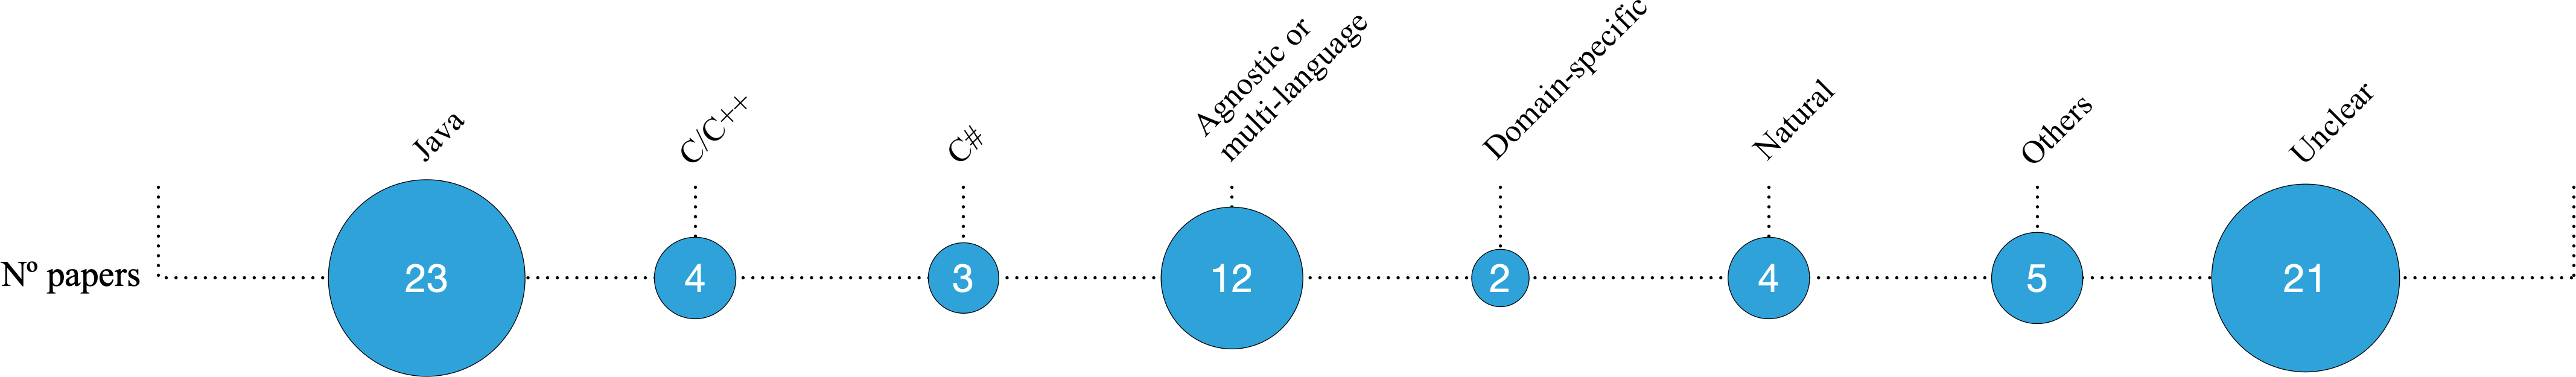
\includegraphics[width=\linewidth]{programming_languages.png}
%  \caption{Distribution of the targeted programming languages.}
%  \label{fig:programming_languages}
%\end{figure}


\begin{tcolorbox}%[size=fbox]%[boxsep=0mm,boxrule=0mm,size=minimal]
%\small
\textbf{Summary of RQ2.}
Our survey shows that a large number of papers exhibit \rea concerns in their motivations, and a smaller albeit still significant amount contains experiments at relevant scale. 
Most of the times, the techniques that are implemented into a software workflow are also papers that have authors from an industrial background. %while transferal of approaches that stem purely from academia still remains a challenge.
Unfortunately, few authors share their tools in a well-documented, open-source fashion, which hampers both future researchers, who wish to compare their solutions against the state-of-the-art, and practitioners, who might want to see how existing \rt tools can help their software.
\end{tcolorbox}






\subsection{RQ3: Evidences of Real-world Application of \\Regression Testing Techniques}
\label{sec:lit_rq3}

Our study is motivated by the concern that there is potentially valuable technology being proposed in academia that does not always make its way into usage in industry.
The difference between the state-of-the-art techniques proposed in academia and the ones actually used in real-world software is what we call the \emph{academia-industry technology transfer gap}.
Expressing concerns over \rea of \rt techniques is an important step towards awareness of the gap, although not sufficient \textit{per se} to solve the problem of actually putting these techniques into practice.
The focus of this section is to discover if and how much evidence exists of techniques developed by the research community being adopted by real-world software development.
As previously stated, there might be studies that have been put into practice, but escaped our review because they were not explicitly motivated by \rea; we hope that, in the future, our live repository solution will eventually find them and potentially widen the conclusions described here.

\autoref{table:relevance} contains only data extracted from the papers themselves; since the author responses are anonymous, we cannot map them directly to the table.
Thus,~\autoref{fig:relevance_count} displays the total number of papers that satisfy each of our applicability criteria, including updates from the author responses.
In other words, we consider the author response if it updates the information retrieved from the paper; otherwise the data extracted from the paper remains.

%\begin{figure}
%  \center
%  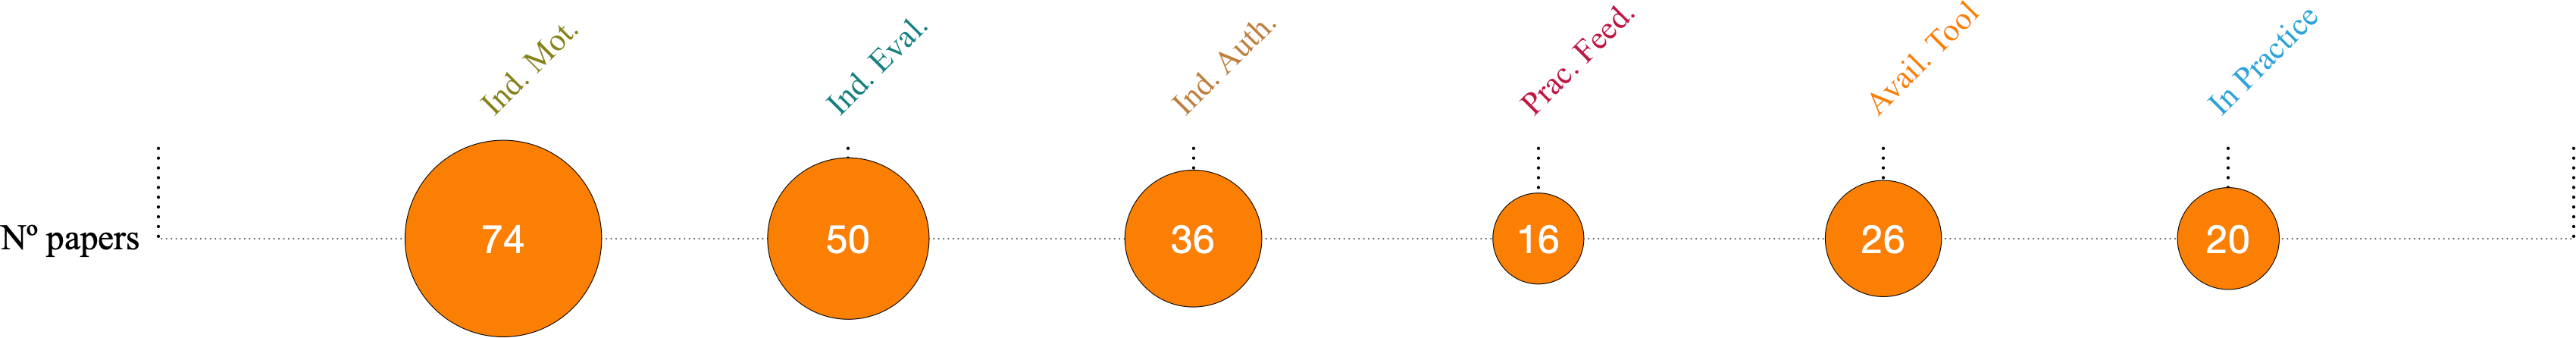
\includegraphics[width=\linewidth]{relevance_count.png}
%  \caption{Quantitative analysis of the satisfied criteria.}
%  \label{fig:relevance_count}
%\end{figure}


Regarding the adoption of the proposed approaches, \autoref{table:relevance} shows that 16 out of the \numpapers selected papers explicitly state that the proposal is applied with a partner, or suggest that implementation was ongoing at the time of publication, out of which six are confirmed to still be in use by their authors, while four say it fell out of use (the remaining six did not respond, so we assume no change).
Eight other authors claim their approach was implemented after publication, so the count in~\autoref{fig:relevance_count} is 20 (16-4+8).

We can observe that having a practitioner as a co-author helps to provide a direct line from the founding theory of the technique to its application in practice: 
indeed, 14 of these 20 papers have at least one author from industry.
This is not surprising, because such collaborations often originate directly from a need expressed by the practitioners.

However, we also see that only 8 out of those 20 papers featured feedback from the practitioners who actually used the developed tool.
That is, although the tool was incorporated into the production workflow, in many cases an assessment of long-term benefits and acceptance by its users is either not done or not reported.
%
Ultimately, the authors were our best chance of understanding the story behind each tool, revealing whether it is still being used by a partner and the reasons it might have fallen out of use.

From the respondent authors, we received six confirmations that the tool continues to be in use by their industrial partner in some form, e.g. ``\textit{The tool was implemented at a company [...] and it is still in use at the company [with significant changes].}'' from respondent author \#14.
Authors of another two papers stated that the technique is undergoing an implementation process at the time of the response.
Author \#37 claims that their work on a newer paper is seeing adoption by an industrial partner; however, at the time of writing, that paper remains in pre-print and cannot be formally included in this review.

Interestingly, eight authors say that the tool was successfully incorporated into an industrial partner's development cycle after the publication of the paper: ``\textit{the technique has been adapted and embedded into a random data selection tool by the [company]’s testing team, for purposes including but not limited to regression testing.}'' (author \#36); ``\textit{the [technique] has been in use at [company since roughly the date of publication. [It] is used to run relevant test cases for every code review in [company]'s main code repository.}'' (author \#23).
However, the details are not always known to them: ``\textit{We were told it was put into practice but we were not given any information, due to confidentiality rules.}'' (author \#44).

To the extent of the authors' knowledge, 12 papers were never put in practice, although some say there was a discussion to do so at some point.
From author \#35: ``\textit{We discussed the possibility of conducting a research visit at one of the corporation branches to experiment with the technique} in vivo\textit{, but in the end it did not go through.}''

Authors of ten papers (out of which four were tagged as implemented in~\autoref{table:relevance}) said that the tool saw usage but fell out of use after a few years; an additional three claimed some sort of attempt, but the current status is unknown.
What this means is that, even if a technique is incorporated into a software, a lot of work must still be done to ensure that the approach remains viable in a longer term.
Some challenges mentioned by these authors include:

\paragraph{The tool became outdated and it was not updated to remain relevant}
``\textit{It was implemented in an industrial setting, but this work is several years old and has to be evolved to stay relevant for business.}'' (author \#20).
This can be either due to a technical issue, e.g. the tool was designed for an older version of a programming language or platform and would require some effort to be updated and be used on newer software, or because the tool does not consider newer requirements of its subject software.

\paragraph{The authors noticed that adapting an academic prototype into an industry-strength tool required more time and budget than the project permitted}
``\textit{There is a gap between developing a research prototype and an industrial-strength tool. Evolving research prototypes towards industry-ready tools was beyond the project budget.}''(author \#8)
It can happen that a technique seems promising in initial experiments, but an enormous amount of work would be needed to actually incorporate it into a workflow.
The technique might require data that is not currently being collected, or use some manual process for the evaluation that would need to be automated.
The tool must also be verified for correctness and robustness before practical usage.

\paragraph{Authors lost contact with their partners and no longer follow development of the tool}
``\textit{[The tool] was supported by [our partner]. We have no input if the tool has been used.}'' (author \#26)
There are cases where the partnership does not continue after the publication of the paper or some other condition occurs.
The industrial partner is likely free to continue using the developed tool, but the authors from the academic side are no longer part of its evolution and do not receive updates and feedback regarding the subsequent challenges and achievements.

\paragraph{The cost-benefit ratio was off}
``\textit{We tried to use it within [our partner]. It seemed to work fine but the cost associated with the 1\% bugs that were missed is too high.}'' (author \#43)
Even if a \tcs technique detects 99\% of bugs by running a very small set of tests, practitioners will be skeptical of using as a replacement for TestAll strategy.
After all, although testing is a costly procedure, it is still much cheaper to detect an error during testing than after the software has been shipped to customers.

%\begin{figure}
%  \center
%  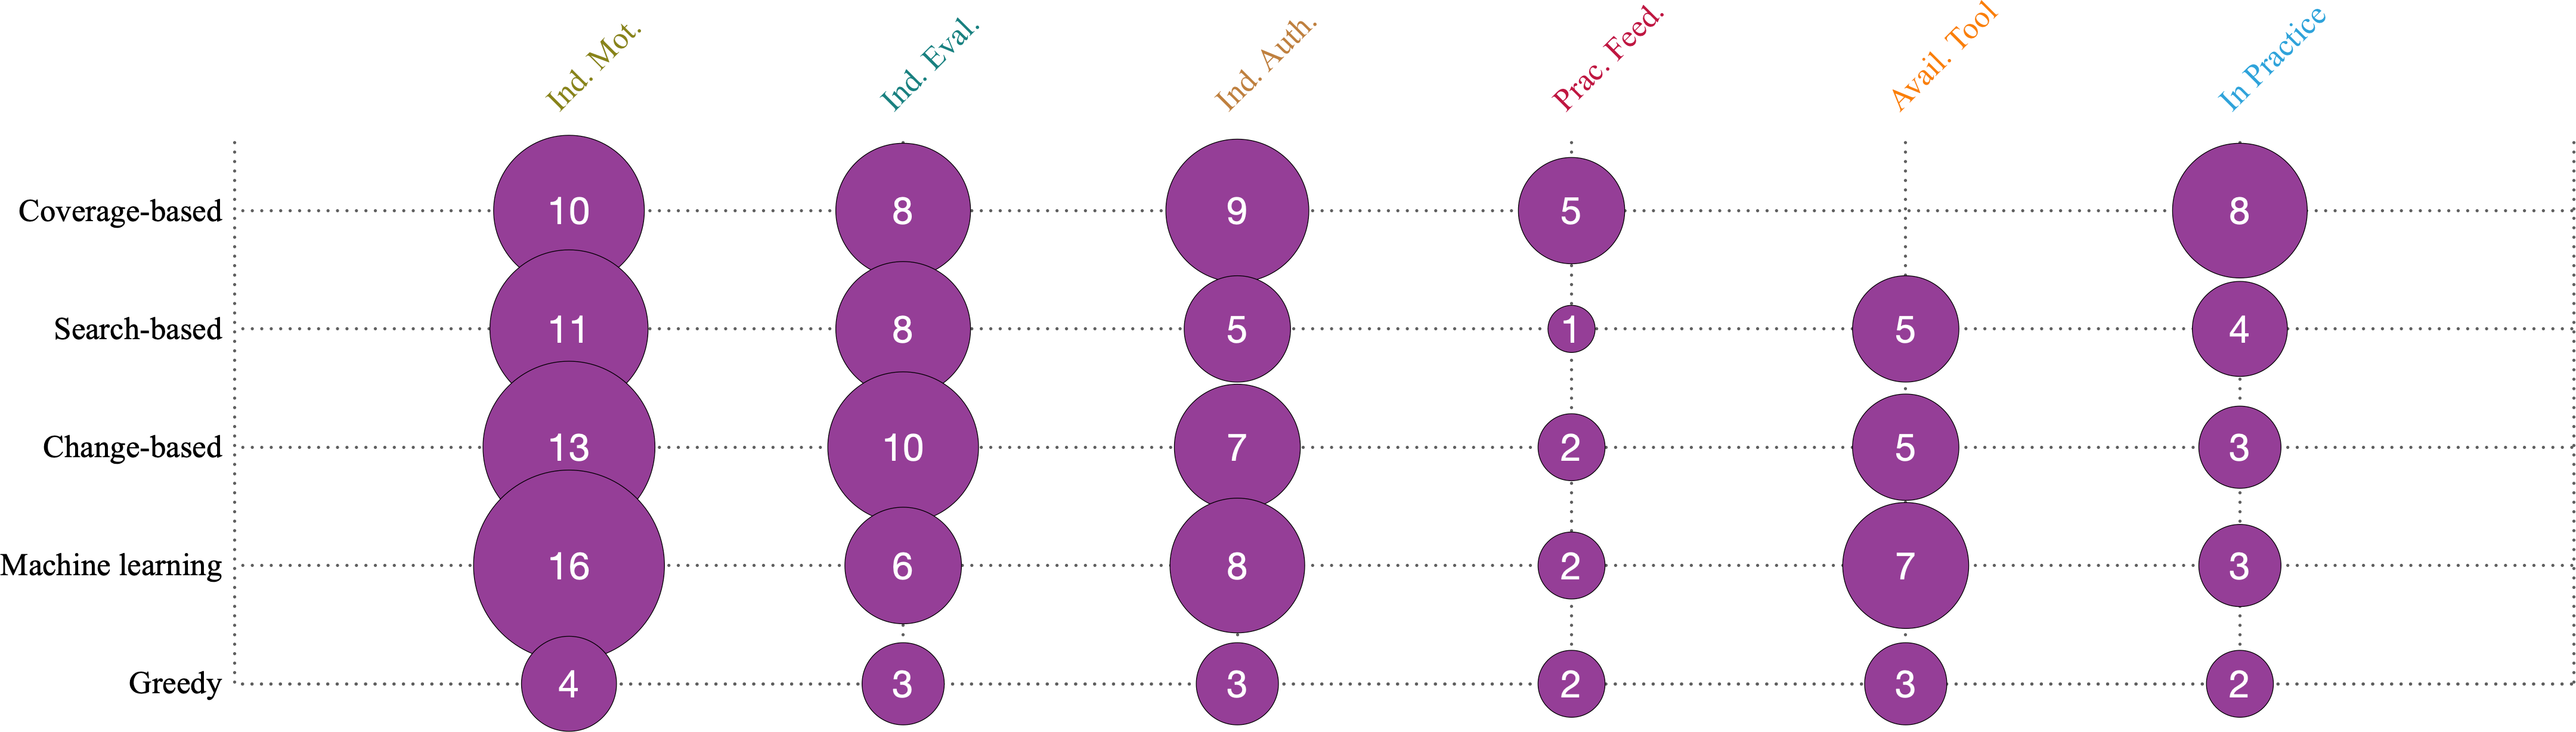
\includegraphics[width=\linewidth]{approaches_applicability.png}
%  \caption{Mapping of approaches and techniques that have seen practical application on at least 2 papers.}
%  \label{fig:approaches_applicability}
%\end{figure}

\autoref{fig:approaches_applicability} shows the relationship between the applicability criteria and the approaches that have seen real-world usage.
The figure shows approaches with at least two papers put into practice\footnote{Constraint-based, graph-based, similarity-based, trace-based, manual classification, cost-aware and history-based approaches have one paper each implemented in practice.}.
Unsurprisingly, the most common information-type and algorithm-type approaches are the ones that see the most real-world usage.
Coverage-based approaches dominate the implementations of techniques, despite previous concerns regarding the cost of measuring coverage \cite{herzigkeynote}; although time-consuming, coverage measurements are easy to obtain in most programming languages.
Conversely, there are 16 papers proposing machine learning approaches, but only three were implemented, likely because machine learning models are only as good as the data they are fed; often, obtaining data of enough volume and quality is more difficult than implementing the method itself.

From the practitioners' point of view, one possible source of information is grey literature --- that is, material produced by experts and published without peer-review.
However, this data is decentralized and unstructured, making it difficult to locate useful information.
We did find one example: Netflix has a post on their blog \cite{netflixlerner} describing a system they developed inspired by \citetalias{spieker_reinforcement_2017}.
This indicates that grey literature might be worthy of investigation, but such an effort would fall beyond the scope of the current study.

To provide some insight into the state of practice, we surveyed 23 practitioners who are involved with software development and/or testing at their workplace.
60\% of respondents claim they do not know about \rt tools that originated from research, which corroborates the well-known lack of communication.
35\% say they use or have used a tool to aid \rt; however most of these claim the tool was developed specifically for their needs, so it is not clear that their origins can be traced back to Software Engineering research.


\begin{tcolorbox}%[size=fbox]
%\small
\textbf{Summary of RQ3.} From the papers and the responses we received, we have evidence that 20 papers propose techniques that are still being used in practice.
It is a relatively small number, but it shows that \rt research can have concrete positive impact on real-world software development.
Unfortunately, many of the techniques that are implemented fall out of use after some time, as an ongoing effort is needed to motivate their usage and keep the tool relevant and updated.
There is a hint of evidence stemming from grey literature, although practitioners themselves, when surveyed, mostly claim to be unaware of \rt techniques originated in academia.
\end{tcolorbox}
